%%%%%%%%%%%%%%%%%%%%%%%%%%%%%%%%%%%%
% KTHEEtitlepage_ex.tex
%
% Example of how to use the KTHEEtitlepage package.
% 
% Mats Bengtsson,  7/8 2006
%%%%%%%%%%%%%%%%%%%%%%%%%%%%%%%%%%%%
\documentclass[12pt,a4paper]{article}
\usepackage[a4paper,left=3cm,right=3cm]{geometry}
\usepackage{filecontents,lipsum}
\usepackage[noadjust]{cite}
\usepackage{graphicx,wrapfig,lipsum}
\usepackage{wrapfig}
\usepackage[nonumberlist,acronym,shortcuts]{glossaries}
\graphicspath{{Images/}}
\usepackage{booktabs}

\usepackage{titlesec, blindtext, color}
\definecolor{gray75}{gray}{0.75}
\newcommand{\hsp}{\hspace{20pt}}
\titleformat{\section}[hang]{\Huge\bfseries}{\thesection\hsp\textcolor{gray75}{|}\hsp}{0pt}{\Huge\bfseries}

\usepackage{pdfpages}

\usepackage{fancyhdr}

\pagestyle{fancy}
\fancyhf{}
\rhead{\rightmark}
\lhead{\leftmark}
\cfoot{\thepage}


\usepackage{textcomp,xspace}
\newcommand\la{\textlangle\xspace}
\newcommand\ra{\textrangle\xspace}
\usepackage[T1]{fontenc}
\usepackage{lmodern}

\usepackage[titletoc]{appendix}
%\usepackage{appendix}
\usepackage{listings,lstautogobble}
\usepackage{color}
\definecolor{dkgreen}{rgb}{0,0.6,0}
\definecolor{gray}{rgb}{0.5,0.5,0.5}
\definecolor{mauve}{rgb}{0.58,0,0.82}
%\definecolor{backcolour}{rgb}{0.95,0.95,0.92}
%\lstset{escapeinside={<@}{@>}}


\definecolor{codegreen}{rgb}{0,0.6,0}
\definecolor{codegray}{rgb}{0.5,0.5,0.5}
\definecolor{codepurple}{rgb}{0.58,0,0.82}
\definecolor{backcolour}{rgb}{0.95,0.95,0.92}

\lstdefinestyle{mystyle}{
    aboveskip=3mm,
    belowskip=3mm,
    backgroundcolor=\color{backcolour},   
    commentstyle=\color{codegreen},
    keywordstyle=\color{magenta},
    numberstyle=\tiny\color{codegray},
    stringstyle=\color{codepurple},
    basicstyle=\footnotesize,
    breakatwhitespace=false,         
    breaklines=true,                 
    captionpos=b,                    
    keepspaces=true,                 
    numbers=left,                    
    numbersep=5pt,                  
    showspaces=false,                
    showstringspaces=false,
    showtabs=false,                  
    tabsize=2,
    escapeinside={<@}{@>},
    language=C,
    autogobble=true
}



\lstset{frame=tb,
    language=C,
    aboveskip=3mm,
    belowskip=3mm,
    showstringspaces=false,
    columns=flexible,
    %basicstyle={\small\ttfamily},
    basicstyle=\footnotesize,
    numbers=none,
    numberstyle=\tiny\color{gray},
    keywordstyle=\color{blue},
    commentstyle=\color{dkgreen},
    stringstyle=\color{mauve},
    backgroundcolor=\color{backcolour}
    breaklines=true,
    breakatwhitespace=true,
    tabsize=3,
    escapeinside={<@}{@>},
    autogobble=true,
    numbers=left,
    stepnumber=5,    
    firstnumber=1,
    numberfirstline=true
}

\lstset{style=mystyle}


\usepackage[exjobb]{KTHEEtitlepage}
%\renewcommand{\cftsecleader}{\cftdotfill{\cftdotsep}}

% Packages used in the main document for this particular example:
\usepackage{url}
\usepackage{tocloft}
\renewcommand\listfigurename{List of Figures}
\renewcommand\listtablename{List of Tables}



\newcommand{\quotes}[1]{``#1''}
\usepackage{hyperref}
\usepackage[all]{hypcap}
%\usepackage{acro}
\hypersetup{%
	pdfborder = {0 0 0}
}
\usepackage[exjobb]{KTHEEtitlepage}

 \newacronym{asip}{ASIP}{Application Specific Instruction-set Processors}
 \newacronym{ebnf}{EBNF}{Extended Backus Naur Form}
 \newacronym{cpri}{CPRI}{Common Public Radio Interface}
 \newacronym{osi}{OSI}{Open Systems Interconnect model}
 \newacronym{gpp}{GPPs}{General Purpose Processors}
 \newacronym{asic}{ASIC}{Application Specific Integrated Circuit}
 \newacronym{tlm}{TLM}{Transaction Level Modeling}
 \newacronym{pla}{PLA}{Programmable Logic Array}
 \newacronym{fpga}{FPGA}{Field Programmable Gate Arrays}
 \newacronym{rbs}{RBS}{Radio Base Station}
 \newacronym{ieee}{IEEE}{Institute of Electrical and Electronics Engineers}
 \newacronym{eda}{EDA}{Electronic Design Automation}
 \newacronym{hdls}{HDLs}{Hardware Description Languages}
 \newacronym{hls}{HLS}{High Level Synthesis}
 \newacronym{rtl}{RTL}{Register Transfer Level}
  \newacronym{crc}{CRC}{Cyclic Redundancy Check}
 \newacronym{fcs}{FCS}{ Frame Check Sequence}
 \newacronym{sfd}{SFD}{Start of Frame Delimiter}
\newacronym{bnf}{BNF}{Backus Naur Form}
\newacronym{uvm}{UVM}{Universal Verification Methodology}
\newacronym{vhdl}{VHDL}{Very High Speed Integrated Circuit Hardware Description Language}
\newacronym{clb}{CLB}{Configurable Logic Block}
\newacronym{drra}{DRRA}{Dynamic Re-programmable Resource Array}
\newacronym{mac}{MAC}{Media Access Control}
\newacronym{pe}{PE}{Processing Element}
\newacronym{srio}{SRIO}{Serial Rapid I/O}
\newacronym{pcie}{PCIe}{Peripheral Component Interconnect Express}
\newacronym{bbu}{BBU}{Base-Band Unit}
\newacronym{ovm}{OVM}{Open Verification Methodology}
\newacronym{vmm}{VMM}{Verification Methodology Manual}
\newacronym{dsp}{DSP}{Digital Signal Processing}
\newacronym{risc}{RISC}{Reduced Instruction Set Computer}
\newacronym{ics}{ICs}{Integrated Circuits}
\newacronym{socs}{SoCs}{System on Chips}
\newacronym{apis}{APIs}{Application Programming Interfaces}
\makeglossaries

\begin{document}
    
\includepdf[pages={1,2}]{cover.pdf}
% Information to appear on the title page:
\ititle{\textbf{Reconfigurable hardware programming  \\ in a   protocol processor unit}\\}
%\isubtitle{Grammar based language framework \\ for hardware/software co-design}
%\isubtitle{}
\iauthor{ - Sunil Kallur Ramegowda}
\idate{2015}

\irefnr{TRITA ICT-EX-2015:206}

\iaddress{ICT Labs\\
	Major in Embedded Platforms\\
		Kungliga Tekniska H�gskolan}
		%\makeititle

		% Everything below is exactly as for a normal document and 
		% the layout of that document should not be affected in any
		% way by the title page.
        
        
        % \section*{}
         \thispagestyle{empty}
        %  \begin{figure}[!htb]
              {\centering
              
\includegraphics[scale=0.45]{logo}\\
              \vskip1.0cm
              Ericsson AB \\
              Department of ASIC/FPGA \\
              Stockholm,Sweden.\\
               \vskip3.0cm}
               
              
               This thesis is carried out in co-operation with Ericsson AB.\\
               
               I would like to thank my manager Mr. Pierre Rohdin G for selecting and providing me with an opportunity to pursue Master thesis at Ericsson. I wish to extend sincere thanks to my senior supervisor Mr. Tume Wihamre for all his guidance and support to make me understand and solve the research question. It is my pleasure to thank my immediate supervisors Katarina Nilsson and Orri Tomasson who helped me all along my thesis by guiding patiently, providing constructive feedback, arranging weekly meetings and reviewing my work. I would also take this opportunity to thank other thesis students Mehdi Taabouri, Jing Zhang X and Marcus Andersson who were next to me all the time, for all the discussions at my work place.                
               
               
               
        %      \caption{}
        %      \label{}
        %    \end{figure}
            
            
            
          \clearpage
        
         \section*{Acknowledgement}
         \thispagestyle{empty}
         
         \vskip1.0cm
         
         First of all I would like to thank Dr. Johnny �berg for being my supervisor and examiner and for his support, guidance and advice throughout the research project. I wish to thank EIT ICT Labs Master school for providing me an opportunity to study Master's in Embedded platforms. I am pleased to thank all the Professors of AES dept, TU Berlin and ICT school, KTH. I extend my gratitude to the coordinators Nina Reinecke at TU Berlin and Helena T�rnkvist at KTH for all the administrative help.\\
    
         Last but not the least, I would like to thank my parents and sisters for their unconditional support, both financially and emotionally throughout my degree. In particular I am grateful for my 2 year old nephew who made them happy all the time in my absence. I would also extend my thanks to all those who sponsored my studies including Vijaya Bank, India. 
         
               
         
         
        
         \clearpage

		\title{Reconfigurable hardware programming in a protocol processor unit}
		\author{Sunil Kallur Ramegowda}

		\pagenumbering{roman}
        
       \phantomsection
       
       \addcontentsline{toc}{section}{Abstract}
        \maketitle
        
       
  		\begin{abstract}
          
        %\normalsize
        \vspace*{3\baselineskip}
		%\vspace*{1in}
        Reconfigurable hardware architectures have been a research topic for many years. Programming such architectures requires manual low level coding or the design of custom compilers to generate the required configuration data for the architecture.\\
        
        In general, a protocol processor processes the packets according to the protocol. There are number of protocols like Ethernet and \acs{cpri} to define how the data has to be sent and received between the source and destination points. Data packets can be processed using generic processors programmed in software, but hardware processing is always faster and energy efficient.\\  
        
        A compiler/mapper is investigated in this thesis work. The language application is developed using a parser generator tool called Antlr. The grammar is written in \gls{ebnf} and the corresponding language is used to describe the architecture and the protocols. The tool will generate a hardware model and its interconnections in SystemC TLM2.0 based on the protocol description. The hardware model is connected to \gls{uvm} driver and functionality is verified by simulation. The Ethernet protocol is described using the developed language and the complete framework is verified.\\ 
      
        
        
        
		\end{abstract}
        
       	\cleardoublepage

        %\renewcommand\contentsname{\centerline{\underline{\underline{Table of Contents}}}}
		\phantomsection
        %\cleardoublepage
        %\addtocontents{toc}{~\hfill\textbf{Page}\par}
        \tableofcontents
        %\cleardoublepage
		\addcontentsline{toc}{section}{\contentsname}
		\cleardoublepage
        
        % abbreviations
        \phantomsection
        \addcontentsline{toc}{section}{Abbreviations}
        \printglossary[type=\acronymtype,title=Abbreviations]
        \cleardoublepage

		\phantomsection
		\listoffigures
		\addcontentsline{toc}{section}{List of figures}
		\cleardoublepage

		\phantomsection
        \listoftables
		\addcontentsline{toc}{section}{List of tables}
		\cleardoublepage
        
     %   \phantomsection
     %   \lstlistoflistings
     %   \addcontentsline{toc}{section}{Listings}
     %   \cleardoublepage

		\pagenumbering{arabic}
         
       \section{Introduction}
       \vspace{1cm}
       \thispagestyle{plain}
      
		A set of rules define the communication strategy between digital systems. There are many rules which make the communication possible between systems. Over the decades, the rules have evolved into standards. \gls{osi} is an international effort to facilitate communications among different manufacturers and technologies. The \gls{osi} reference model partitions communication systems into 7 abstraction layers. It addresses the interconnection requirement of an open systems environment.
        
 %       \begin{figure}[!htb]
 %           \centering
 %           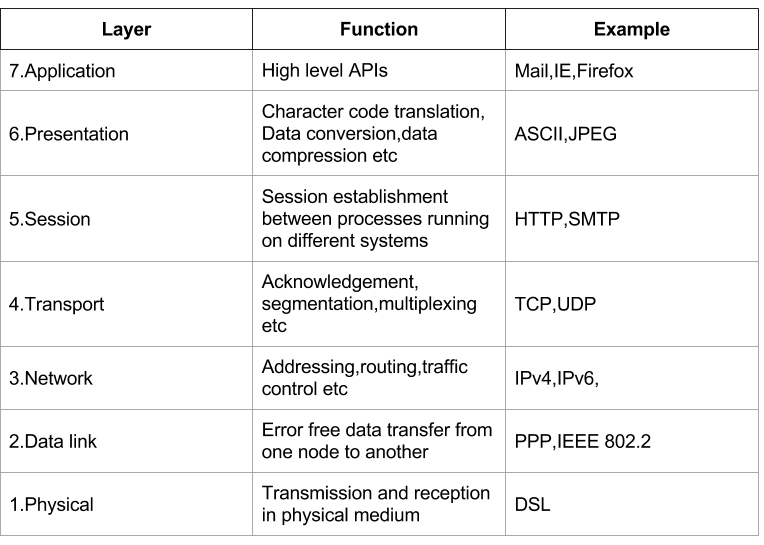
\includegraphics[scale=0.45]{osi}
 %           \caption{OSI Model}
 %           \label{fig:osi}
 %       \end{figure}
        
        
      % Please add the following required packages to your document preamble:
      % \usepackage{booktabs}
      \begin{table}[!htb]
          \centering
          \begin{tabular}{@{}cllc@{}}
              \toprule
              \multicolumn{2}{c}{{\bf Layers}} & \multicolumn{1}{c}{{\bf Functions}}                                                                                 & {\bf Examples}  \\ \midrule
              7         & Application          & High level APIs                                                                                                     & Mail, IE, Firefox \\ \midrule
              6         & Presentation         & \begin{tabular}[c]{@{}l@{}}Character code translation,\\ Data conversion,\\ Data compression etc\end{tabular}       & ASCII, JPEG      \\ \midrule
              5         & Session              & \begin{tabular}[c]{@{}l@{}}Session establishment between \\ processes running on different \\ systems.\end{tabular} & HTTP, SMTP       \\ \midrule
              4         & Transport            & \begin{tabular}[c]{@{}l@{}}Acknowledgement,\\ Segmentation,\\ Multiplexing etc\end{tabular}                         & TCP, UDP         \\ \midrule
              3         & Network              & \begin{tabular}[c]{@{}l@{}}Addressing, Routing,\\ Traffic control etc\end{tabular}                                   & IPv4, IPv6       \\ \midrule
              2         & Data Link            & \begin{tabular}[c]{@{}l@{}}Error free data transfer from \\ one node to another\end{tabular}                        & PPP, IEEE 802.2  \\ \midrule
              1         & Physical             & \begin{tabular}[c]{@{}l@{}}Transmission and reception in\\ physical medium.\end{tabular}                            & DSL             \\ \bottomrule
            \end{tabular}
            \caption{OSI Model}
            \label{osi}
        \end{table}
        
       
        The rules are referred as \textit{protocols} in communication systems. They help in the exchange of information between the digital systems. Most of the higher layers (4 to 7) are processed through generic computer systems and the lower layers with dedicated embedded hardware. \gls{gpp} found in embedded systems cover a broad range from 8 bit low cost microcontrollers, to 32 bit RISC microprocessors, to today's high performance processors with \gls{dsp} enhancements.  They can be considered as hybrid processors which incorporate signal processing features into embedded hardware that unify control and signal processing in a single core. In the communication domain, a network processor is a programmable microprocessor optimized for processing network data packets. Common functions include header parsing, pattern matching, bit manipulation, packet modification, shift and data movement. Software programmability of network processors allows it to be more flexible across a range of applications. Even though all network processors are programmable, the user might not be given access for programming, restricting the programmability to vendors. Other \gls{gpp} can be programmed for protocol processing as they are less expensive. Solutions based on \gls{gpp}  or \gls{asic} exist \cite{5335678} \cite{558379} for protocol processing. GPPs will have more flexibility but are less energy efficient when compared to \acs{asic} which is less flexible but the most energy efficient. \gls{asip} or domain specific processors are more suitable for the protocol processing task and depending on their architectural characteristics they allow varying degrees of trade-off between flexibility and energy-efficiency \cite{1106752}.\\   

	     Another class of hardware architecture referred as Reconfigurable architecture, are devices that contain programmable function blocks and programmable interconnects between function blocks. The most mature class of reconfigurable architectures is \gls{fpga} which are considered fine-grained reconfigurable architectures. Research advances in this field have led to the Coarse grain re-configurable architectures and reconfigurable computing platforms. Hardware resource usage and performance varies depending on the reconfigurable architecture and its level of abstraction \cite{6868627}. The design of coarse grain reconfigurable hardware architecture requires the compiler to produce the configuration or the hardware compatible code \cite{5681536}. These files can be produced at run time when the application is running or in a static way before execution. The complexity of the system depends on the selected design.\\ 

		The reconfigurable hardware is modeled in SystemC language using \gls{tlm}. The files required for the reconfiguration are obtained by parsing the description of protocols which is described in high level language. The Antlr tool is used for building the base parser file for the defined grammar and then the required functions are implemented to output the complete system and configuration data. 
        

		
	%	\subsection{Background}
        
        \subsection{Hardware and programming}
        
        Until the late 1960s, \gls{ics} were designed, optimized, and laid out by hand. Gate level simulation appeared in the early 1970s, and cycle based simulation became available by 1979. Place and Route, schematic circuit capture, formal verification and static timing analysis techniques were introduced during the 1980s. Meanwhile Gajski and Kuhn introduced the Y chart for describing  
        the hardware as 3 different domains namely \textit{Behavioural Domain}, the \textit{Structural Domain} and the \textit{Physical Domain} \cite{1654264}. It represents different levels of hardware abstraction which are indicated by concentric circles as illustrated in  Fig.~\ref{fig:Gajski}. The three axes represents the 3 different domains and the synthesis can be viewed as a process of transformation from one axis to another and/or from higher level to lower level. The behavioural domain describes the functional behavior of the system. The structural domain maps the hardware into subsystems and show they are interconnected. The geometrical domain represents the geometric properties of the system and its subsystems. Each intersection point of domains and concentric circles represents different abstraction levels with respect to their domains. Simulation tools to represent the hardware are widely adapted during 1980s based on hardware description languages such as Verilog(1986) and \gls{vhdl}(1987).\\ 
        
        
        \begin{figure}[!htb]
            \centering
            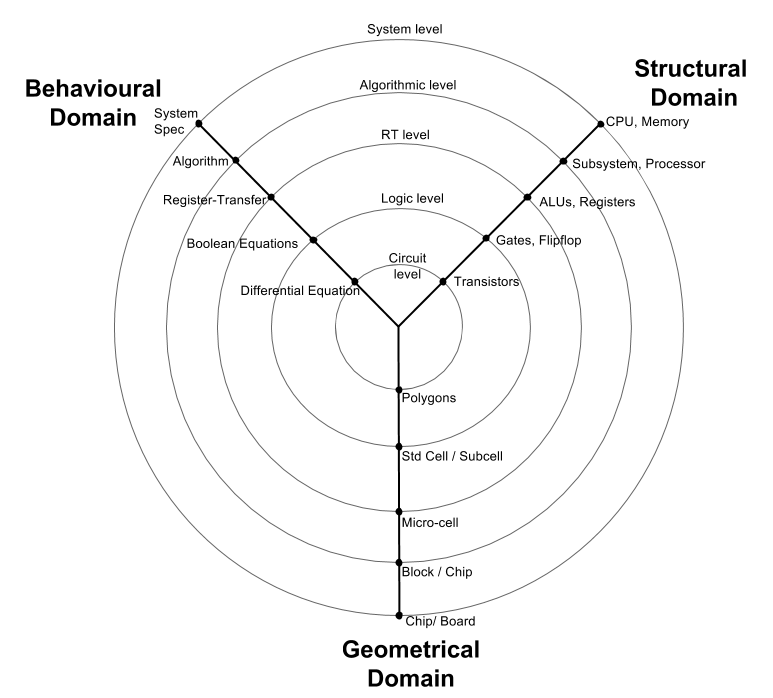
\includegraphics[scale=0.55]{Gajski}
            \caption{Domains and level of description in Gajski Y-chart}
            \label{fig:Gajski}
        \end{figure}
        
        
        In the software domain, similar to the hardware domain, progress in design methodologies for programming the hardware has helped with today's sophisticated hardware independent compiler environment. Machine code was once the only means of programming the hardware. In 1950s, assembly level programming was introduced which abstracted the programming one step higher. With the compilers becoming more intelligent, high level languages evolved and associated compilation techniques were developed to improve software productivity. High level languages like Python, Perl, Java, PHP etc are platform independent and provide the user with flexibility and  portability by hiding details of hardware architecture. Languages like C, C++ abstracts from assembly level, and together with C compilers, it helps in efficient object code generation. Programmers create interfaces to the C library so the routines can be used from higher level languages. With the new hardware architecture becoming more complex in nature, the software applications are developed to provide good solutions which are in parallel becoming more complex. 
        
        \subsection{Reconfigurable systems} \label{reconf}
            
            	In 1960, Gerald Estrin proposed the idea of a fixed plus variable structure computer \cite{1114865}. It consisted of a fixed processor and an array of reconfigurable hardware which was controlled by the fixed processor. Even though the idea was demonstrated with a proof, the industry did not consider to further innovate in this field and till the 1980's there were no significant developments. In  1985, the reconfigurable \gls{pla} was patented \cite{page1985re}. Innovation in \acs{pla}s further continued with the commercially available \gls{fpga} in today's market.\\
                
                
            In the field of computer architecture, designers make decisions based on flexibility and performance requirements \cite{JACST518}. \acs{asic}s are the least flexible in terms of adapting for any change in the application, and GPPs are the most flexible as they are independent of the application and the core can be programmed to make the required algorithm work at the cost of higher power and lower efficiency. ASIC and GPP lie in the extreme corners of the graph between flexibility Vs performance as shown in Fig.~\ref{fig:Fig1}. Reconfigurable architectures are intended to fill the gap and provide more flexibility in terms of hardware and potentially higher performance than software \cite{JACST518}.
            
            \begin{figure}[!htb]
                \centering
                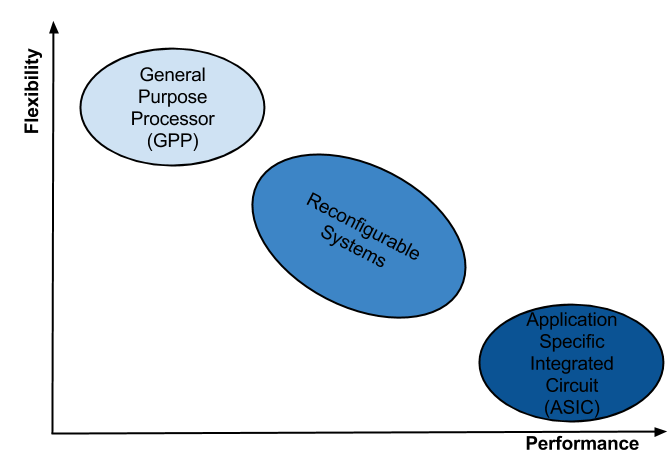
\includegraphics[scale=0.45]{Fig1}
                \caption{Flexibility Vs performance of hardware classes}
                \label{fig:Fig1}
            \end{figure}
            
            \subsubsection{Granularity} 
            
            Reconfigurable devices like \acs{fpga} have the \gls{clb} which can be configured to map the required functionality. The complexity of the function is not a concern, but the number of inputs and output of the function have to be considered based on the FPGA architecture. This level of granularity in implementing the functions is called Fine grained Reconfigurable Architecture as it provides the reconfigurable granularity to lowest possible level. These reconfigurable devices are not energy efficient and the execution speed is less than the ASIC counterpart. Another type of reconfigurable devices are the coarse grained reconfigurable architectures. These devices have the granularity at function level. They will configure the function blocks to achieve efficient algorithm implementation. The function blocks can vary from constant blocks to complex functions which are commonly used by the application.   
            
            
            \subsubsection{Reconfiguration models}
            The reconfigurable architectures need configuration of hardware. This can be at compile time or at runtime of an application as in  Fig.~\ref{fig:Fig2}.
            
            \begin{figure}[!htb]
                \centering
                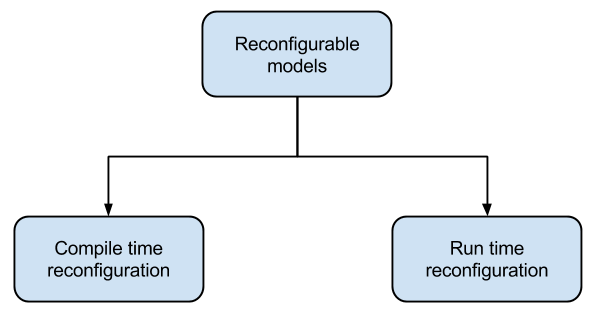
\includegraphics[scale=0.5]{Fig2}
                \caption{Reconfiguration models}
                \label{fig:Fig2}
            \end{figure}
            
            In the compile time reconfiguration model, the reconfigurable hardware system is configured at compile time and will be static during the application run time. In this model the programmable logic can be configured to perform some specific task like hardware accelerators to achieve high performance. An FPGA configured to perform floating point multiplication together with a GPPs will accelerate the performance of the application if the GPPs doesn't have a Floating Point Unit.
            In the run-time reconfiguration model, the reconfiguration hardware is configured at run time and will be dynamically programmed to perform different tasks. The decision for making such dynamic reconfiguration has to be embedded coupled with the application and hence it increase the overhead. The \gls{drra} fabric developed at KTH Electronic System Dept is an example of this model \cite{5351593}.   
            
            \subsubsection{Reconfiguration rate}
            The Fine graine systems will have more reconfiguration data (in FPGAs, it is in term of bit streams), which leads to more configuration time and the Coarse Grained Reconfigurable systems will have comparatively less blocks as they have higher granularity and will contain less reconfiguration data. Hence, the Coarse grain architecture will take less time to reconfigure. This depends on the dynamic reconfiguration architecture whether the complete fabric is reconfigured or partially reconfigured during runtime. 
        
        
		\subsection{Purpose of this thesis}
        
        Ericsson AB \cite{ericsson} is a market leader in the radio base station equipments. There are different protocols being used for communication in the Radio Base Station (RBS) units. Ethernet, explained by \gls{ieee} in 802.3 standard, defines the protocol for 10Gbit transfer which is mainly used for communication between the silicon chips. Other protocols include \gls{cpri}, Serial Rapid IO (SRIO), Xio-s (Ericsson Specific protocol) for reliable communication between chips at high data rate. Most of these \gls{mac} layer protocols share common hardware functions. Ericsson design and manufactures custom \acs{asic} chips for Baseband signal processing and Radio signal processing. The data is received and transmitted from these chips by one of the agreed protocols. A reconfigurable hardware can be designed to route the data using different protocols.\\
        
        The reconfigurable architecture requires a new hardware and software co-design. The reconfiguration details are extracted based on the hardware design and the compiler/mapper should be able to produce such reconfiguration. This is accomplished  by using a Grammar based technique i.e by defining a language based on \gls{ebnf} grammar, and then describing the protocols using this language. The overall architecture and working principle will be explained in further chapters.\\
        
        The thesis deals with understanding the reconfigurable architecture and identifying the configuration details to make the system work for different protocols. The description in high level language is used to extract these configuration details and to verify the complete system using a test bench.\\   

		The purpose of this thesis is to investigate an approach of a compiler or mapper to describe the protocols in high level language and then map it to hardware blocks and their interconnection. This involves showing the proof of concept by SystemC TLM simulation models. The individual hardware blocks are modeled in SystemC TLM and can vary from a simple block to complex functions of the protocols. This thesis work serves as a proof for the project in Ericsson AB to further investigate the feasibility of developing such architectures.


        \subsection{Problem description}
            As explained in the previous section reconfigurable architectures with low granularity are available for different applications. They still face the challenges of lower speed, high energy consumption and the compatibility of tool chains between different vendors. The lowest reconfigurable granularity can be designed at bit, block or function level. When targeting hybrid architectures to improve either performance, cost or speed, the application must be partitioned in such a way that certain repetitive or computation intensive functions are mapped on a reconfigurable hardware. Such mapping is not simple as it requires deep understanding of both hardware and software design \cite{1395538}. The know-how of the process to build the complete system which solves the practical problems is of great importance. Fig.~\ref{fig:designgap} from the International Technology  Roadmap for semiconductors shows how hardware and software design productivity has lagged Moore's law. The need of configuration data for the reconfigurable hardware requires the design of new software tools.\\
            
             \begin{figure}[!htb]
                            \centering
                           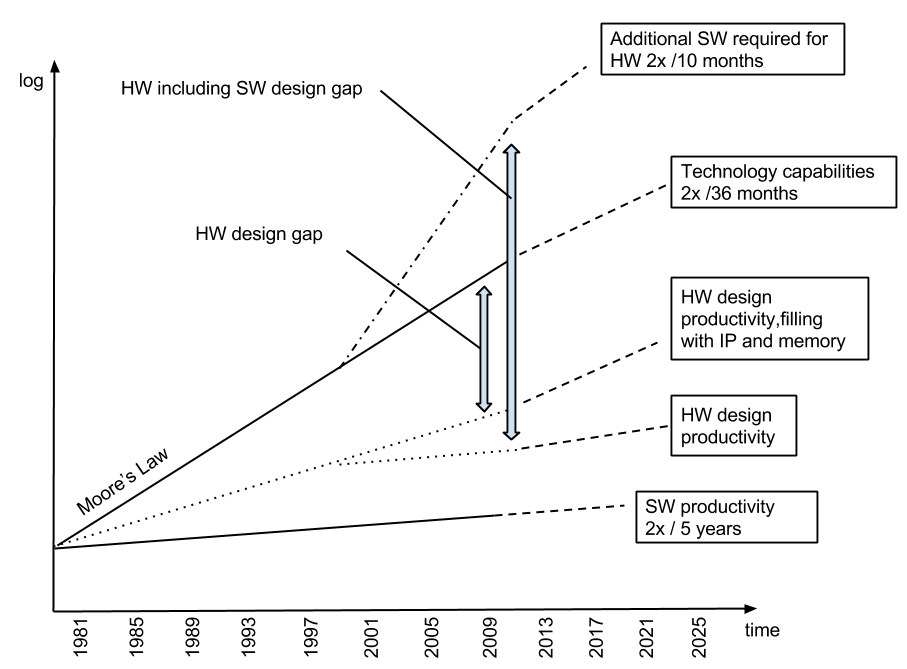
\includegraphics[scale=0.45]{designgap}
                            \caption{Hardware Software Design Gaps versus Time \cite{book}.}
                            \label{fig:designgap}
             \end{figure}
            
            
            
             The \acs{rbs} receives and transmit data using different protocols. Identifying errors and providing security are some of the main features for reliable communications. Algorithms used by different protocols for providing such features differ by minor polynomial change. Identifying such functions is required for efficient reconfigurable hardware design. The designer needs to have the overall understanding of hardware and software for such a system. How the reconfigurable hardware can be programmed to accomplish the protocol processing in an efficient way by designing the framework using high level description needs to be explored. High level language development provides flexibility for the designer to produce reconfiguration data in their own syntax. The development time needs to be evaluated for such an approach.  This allows the user with minimal know how about hardware to reconfigure and show results in short time.

		\subsection{Goals}
		The thesis goal is to achieve the below milestones:
        
        \begin{itemize}
            \item{Understand the reconfigurable hardware architecture designed at Ericsson AB.}
            \item{Understand Ethernet, Xio-s and CPRI protocols.}
            \item{Define a language to describe the protocols in high level description.}
            \item{Identifying how to represent the reconfiguration information.}
            \item{Mapping the description of language to hardware and interconnections.}
            \item{Integrating Ethernet protocol for the complete system.}
            \item{Verifying the system by simulation.}
            
            
        \end{itemize}

		\subsection{Limits on scope}
		The thesis focuses more on showing the proof of concept considering one to two protocols i.e Ethernet and Xio-s. The language will be designed such that it is easy with minor modification to extend for other protocols like CPRI. Developing and integrating the \acs{tlm} models for all the protocols will not be feasible in this time line. The architectural changes required are suggested but not changed as the focus is more on describing the protocol in high level description.

		\subsection{Structure of the thesis}
		The thesis is organized to provide the required details for understanding the overall work. The first chapter gives a brief introduction to the reader about the topic of investigation, limitations and goals. The rest of the thesis is structured as follows.\\
        
        
        \textbf{Chapter 2 :}  This chapter  will describe the background about the topic. It is summarized in three sections starting with Reconfigurable hardware architectures and their terminologies. The three different protocols considered in protocol processors are discussed in detail.\\
        
        
       \textbf{Chapter 3 :}  This chapter starts with the introduction of system design languages.  The complete details of different hardware modeling languages, their comparison and verification methodology is discussed. The later section explains the meaning of a Grammar, the Language and the Parser in computer science world. Then the process of building a language application is explained using Antlr tool.\\
        
        \textbf{Chapter 4 :}  The chapter starts with the comparison of three different protocols discussed in background. The next section explains the complete details of Freyja architecture. It also discusses how the architectural requirements are mapped using the high level description. Mapping of Freyja operators, their memory contents, interconnections and error handling are discussed.\\
        
         \textbf{Chapter 5 :}  This chapter explains the integration of Ethernet protocol functions into the  system of files auto generated from the language application. The challenges and the mapping of input description are discussed in detail. The Xio-s protocol is also considered but part of the functions are integrated to show the context switching and to highlight the control block changes.\\
        
        \textbf{Chapter 6 :}  This chapter explains the details of complete test system. How the overall system can be represented using the input file and how the data is processed and handled within the system.\\
        
              
        \textbf{Chapter 7 :}  This chapter concludes the thesis by explaining the outcome of connecting three dots namely reconfigurable hardware, protocols and High level description. The limitations encountered and the future work is discussed further.
        
          
		\clearpage


		\section{Background}
        \vspace{1cm}
        \thispagestyle{plain}
		To understand the reconfigurable hardware and its terminologies, this chapter explains in detail about different architecture classes and their meaning. Protocols and their common functions are also explained, which helps in designing the reconfigurable protocol processor.   

       \subsection{Fine grain reconfigurable systems}
       
        Fine grain reconfigurable logic arrays have evolved into commercially available \acs{fpga}s. They are a scalable chip architecture based on a 2D array of simple computational cells with individually configurable processing functions and an electronically configurable interconnect structure allowing complex application circuits to be built from the available cells \cite{5382069}.  
        
        \begin{figure}[!htb]
            \centering
            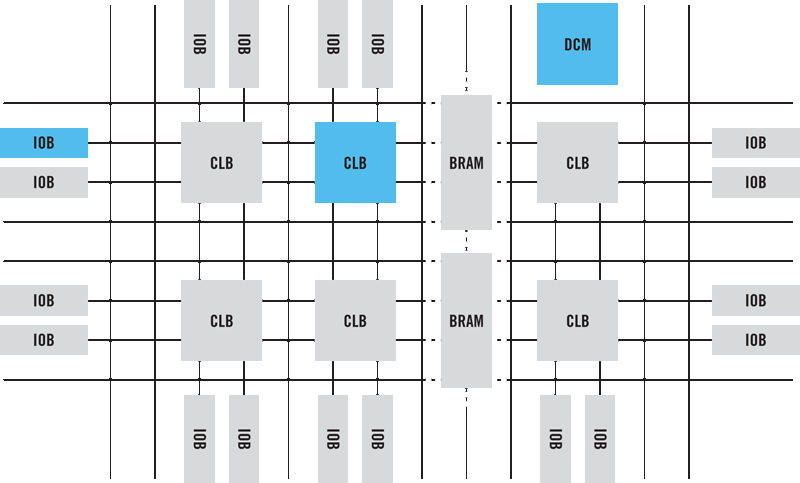
\includegraphics[scale=0.45]{fpga}
            \caption{Field Programmable Gate Array \cite{xilinx}}
            \label{fig:fpga}
        \end{figure}
        
        
        Fig.~\ref{fig:fpga} shows the FPGA architecture with a matrix of \gls{clb} connected through programmable interconnects. The \gls{clb} is the basic logic unit in a FPGA wherein the number of such units in each device varies depending on cost. Each \gls{clb} consists of a configurable switch matrix with 4 or 6 inputs, some selection circuitry and flip-flops. The highly flexible switch matrix can be configured to handle combinatorial logic, shift registers or RAM \cite{xilinx}. IOBs refers to the Basic select IO structure. The interconnect routes the signals between CLBs and to and from IOs. Most of the modern FPGA boards include the Embedded block RAM and Digital Clock Management (DCM).\\  
        
        
         \begin{figure}[!htb]
             \centering
             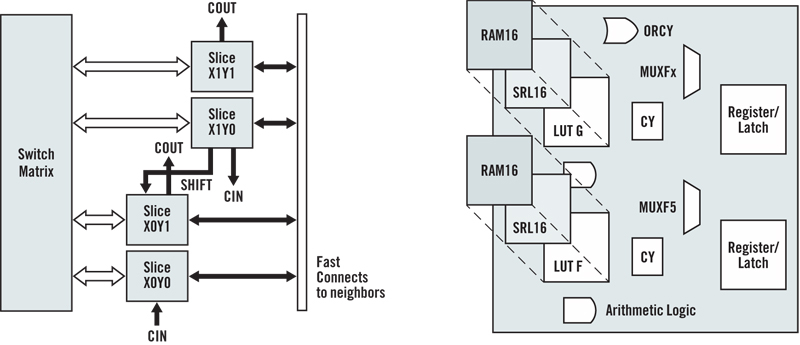
\includegraphics[scale=0.55]{clb}
             \caption{Configurable Logic block \cite{xilinx}}
             \label{fig:clb}
            \end{figure}
        
        
        The introduction of \acs{fpga} led to the research of optimizing and reusing the reconfigurable logic blocks. The  \gls{eda} tools compile and synthesize \gls{hdls}  to create a physical design in terms of the \acs{fpga}'s resources. They are attractive compared to the ordinary CPUs because of less power consumption per computation and price per performance \cite{839320}. Despite these merits, FPGAs have still achieved limited applicability in industries. The main reason is that most software programmers lack the knowledge of hardware description languages which are used to describe the complex algorithms in FPGAs. FPGA programming requires a more rigorous development process, involving training the programmers beyond application level, resulting in an increase in development cost and time to market.\\
        
        To overcome the problems stated above, research on mapping high level description to \gls{rtl} level started. The growing capabilities of silicon technology and the increasing complexity of applications in recent decades have also forced design methodologies and tools to move to higher abstraction levels. The methodology is called \gls{hls}. It enables the automatic synthesis of high level, untimed or partially timed specification (SystemC) to a low-level cycle accurate \acs{rtl} specifications for efficient implementations in ASICs or FPGAs.  During the 1990s, the first generation of commercial HLS tools were available  \cite{5209958}. HLS tools helped the designer to use High Level Languages (HLLs) for FPGA programming similar to processor programming. The latest generation of HLS tools, in most cases, uses either ANSI C, C++, or languages such as SystemC that add hardware-specific constructs such as timing, hardware hierarchy, interface ports, signals, explicit specification of parallelism, and others \cite{5209958}. Some of the commercial HLS tools are Mentor's Catapult C, Forte's Cynthesizer, Cadence C-to-Silicon, NEC's CyberWorkbench and a new French company \textit{Synflow}  tool has its own language named Cx.\\
        
        FPGA requires the reconfiguration of programmable fabric either before the program execution or partial reconfiguration on the fly when the program is running. The streaming and multimedia application requires the reconfiguration of fabric on the fly to optimally utilize the fabric. As FPGAs have granularity at the lowest possible bit level, the reconfiguration data is huge and the time for the hardware to reconfigure increases with the complexity. Most of the data handled in real world is either in byte or word width and reconfiguring the interconnect at bit level can be abstracted to higher level. This reduces the overhead of reconfiguring each bit. Similarly, the commonly used combinatorial logics can be defined as standard blocks for the custom design with the standard set of reconfiguration details. These features will reduce the amount of data and time required for reconfiguration and such a hardware class is called Coarse Grain Reconfigurable Logic.   
        
         \subsection{Coarse grain reconfigurable systems} \label{cgr}
       
         To overcome the limitations of Fine grained reconfigurable systems, new architectures were explored. Optimally designed processing elements which perform word level data processing are configured with few configuration bits at word level. Due to the word level reconfiguration, a small number of configuration bits is required, resulting into a massive reduction of configuration data, memory needs, and reconfiguration time \cite{cgra}. Even the interconnections, since they are grouped in buses, they are configured by a single control signal instead of separate control signal for each wire. Also, because few programmable switches are used for configuration purposes and the \gls{pe}'s are optimally-designed hardwired units, high performance, small area, and low power
         consumption are achieved \cite{cgra}.\\
         
         \begin{figure}[!htb]
             \centering
             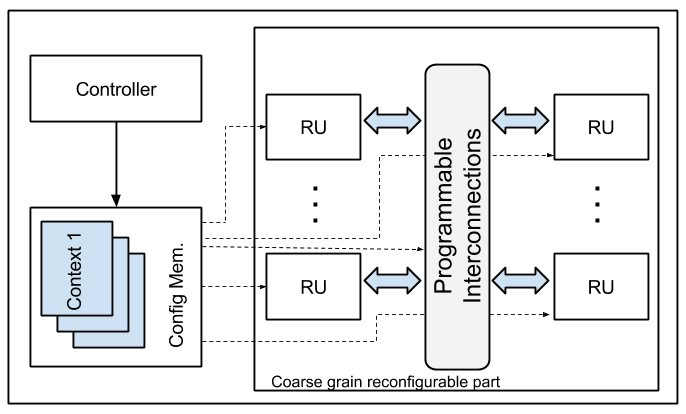
\includegraphics[scale=0.55]{basic}
             \caption{Basic Coarse grain reconfigurable architecture \cite{1303110}}
             \label{fig:basic}
            \end{figure}
         
         
         A generic architecture of a Coarse grain reconfigurable system is illustrated in Fig.~\ref{fig:basic}. It consists of a set of Reconfigurable units (RU), a programmable interconnect, a configuration memory and a controller. The coarse grain reconfigurable part will be designed to take the computationally intensive parts of the application, and in most cases will be coupled to the main processor which takes control of other tasks. Coarse grain architectures are always optimized for the target domain. The number of reconfigurable units, their design, the interconnection network, memory and controller are tailored to the domain's needs. The memory will hold the control (configuration information) bits that are used to program the reconfigurable units and interconnection network. The configuration memory may store multiple configuration contexts but only one context is active at a time \cite{cgra}. The controller is responsible to control the loading of the configuration context from the main memory to the configuration memory, to monitor the execution process of the reconfigurable hardware and to activate reconfiguration contexts.\\
         
         The programmable interconnection network ensures the communication of data between the computing reconfigurable units. The wires are grouped into buses and are configured by single configuration bits. The interconnection network can be realized by a crossbar, mesh or a mesh variation structure.\\
         
         The reconfigurable units are the processing units, which are domain specific hardwired units, perform useful operation to accomplish the application requirements. The operations might refer to logic or arithmetic operation. They reconfigure autonomously based on the control information and are therefore different from the CLB's of fine grain architecture. Each unit is configured at word level, configuration bits reconfigure the entire unit and not each slice at bit level. Theoretically, the granularity might vary from bit to any word length. In most of the practical architectures which are designed, the granularity is either 8bits or above, as the processing of data happens with the word length of 8bits or more. \\
         
         The reconfigurable units in the architecture are optimized hardware units for the application domain. They can be designed to perform any word level arithmetic or logical operations. As coarse grain reconfigurable systems target a specific domain, the RU's are designed with the operation required by the domain in mind. The reconfigurable units are hardwired units optimized to perform for specific application domain to improve performance, area and power consumption.\\
         
         The \acs{gpp} with programmed embedded software is the classical approach which tightly couples data and control flow for many applications. It can be coupled with the general purpose embedded processors in different ways. The design depends on the performance and requirements of the application. Three different scenarios are illustrated in Fig. \ref{fig:cgra}. These additional hardware units coupled to the processor will accelerate the performance or increase the throughput of the overall system. This illustration also helps to understand the different ways of reconfiguring the fabric.         
         
       
       \begin{figure}[!htb]
           \centering
           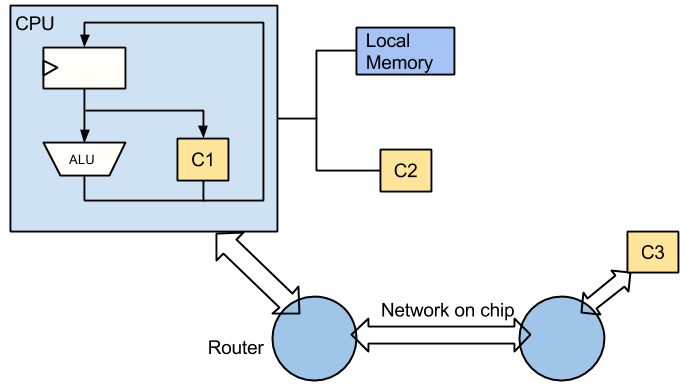
\includegraphics[scale=0.45]{cgra}
           \caption{Coarse Grain Reconfigurable blocks \cite{1303110}}
           \label{fig:cgra}
        \end{figure}
        
        
        Register mapped reconfigurable blocks give the tightest integration with embedded software. They are created by modifying the micro-architecture of the embedded core. For example as in Fig. \ref{fig:cgra}, C1 is an additional data path next to ALU. For programming such an architecture, it should be visible in the instruction set of the embedded core. Since it requires tight coupling, exploiting the parallelism with the introduction of a new hardware unit becomes cumbersome. The tools need to provide such features for the user to map the application to the new hardware architecture. \\           
        
        Memory mapped reconfiguration is the next variant illustrated as C2 in Fig. \ref{fig:cgra}. This is achieved by providing a memory interface to the reconfigurable block. It results in looser coupling between the software and the reconfigurable block. A set of shared memory locations can convey control and data flow orientated information. As explained in \cite{1303110}, reconfigurable blocks need to share memory address space with other peripherals. The control and data flow information might need to be routed through the CPU which increases the bottleneck.\\
        
        In Network mapped reconfigurable blocks (C3), the network packets have the control and data flow information. In this case integration of embedded software and reconfigurable blocks can be done using communication primitives.  As discussed in \cite{1303110}, Network mapped systems deviate more from the classic sequential model and hence the programming model is more complicated. Table.\ref{cgra}  shows the comparison of different coarse grain reconfigurable systems.\\ 
          
         \begin{table}[!htb]
            \centering
            \resizebox{\textwidth}{!}{%
                \begin{tabular}{ccccc}
                    \hline
                    {\bf Mapping} & {\bf \begin{tabular}[c]{@{}c@{}}Architecture \\ Strategy\end{tabular}} & {\bf \begin{tabular}[c]{@{}c@{}}Reconfiguration\\  Mechanism\end{tabular}} & {\bf \begin{tabular}[c]{@{}c@{}}Data flow / \\ Control flow \\ Coupling\end{tabular}} & {\bf \begin{tabular}[c]{@{}c@{}}Energy \\ Efficiency\\  Improvement\end{tabular}} \\ \hline\\
                    \begin{tabular}[c]{@{}c@{}}Register-\\ Mapped\end{tabular} & \begin{tabular}[c]{@{}c@{}}Custom \\ Datapath\end{tabular} & \begin{tabular}[c]{@{}c@{}}Custom \\ Instructions\end{tabular} & \begin{tabular}[c]{@{}c@{}}Tightly\\  Synchronized\end{tabular} & Low \\\\
                    \begin{tabular}[c]{@{}c@{}}Memory-\\ Mapped\end{tabular} & Co processor & \begin{tabular}[c]{@{}c@{}}Memory mapped \\ instructions\end{tabular} & \begin{tabular}[c]{@{}c@{}}Loosely \\ Synchronized\end{tabular} & Medium \\\\
                    \begin{tabular}[c]{@{}c@{}}Network-\\ Mapped\end{tabular} & Peer processor & \begin{tabular}[c]{@{}c@{}}Configuration\\  Packets\end{tabular} & Uncoupled & High \\ \hline
                \end{tabular}
            }
            \caption{Coarse Grain Reconfiguration Mechanism \cite{1303110}}
            \label{cgra}
        \end{table}
        
        
        \subsection{High level synthesis}
        
        High level synthesis is the process of translating from algorithmic to Register transfer level description as illustrated in  Fig.~\ref{fig:Gajski}. Transforming application level programs which are described in high level languages directly into register transfer level will not require the programmer to know the detailed hardware architecture. High level synthesis tools explore the design space based on information from the high level abstraction with more degrees of freedom. There are many academic and industrial projects showing the concept of \gls{hls} \cite{4291932} \cite{5469564}. They operate on internal models known as Control/Data Flow Graphs (CDFG) and produce a \gls{rtl} model of the hardware implementation \cite{998629}. The computationally intensive applications like \gls{dsp} algorithms were the target in the initial research of HLS tools.\\ 
        
        A brief introduction to the academic and industry standard high level synthesis tools is discussed here.\\ 
        
        GAUT \cite{gaut} is an academic High level synthesis tool dedicated to Digital signal processing applications. It is an open source tool which takes a pure C function along with the constraints to extract the potential parallelism and data dependencies. After the allocation, scheduling and binding tasks it will generate the RTL code. \\
        
        Cynthesizer \cite{5209958} is a pin and protocol accurate SystemC model used as synthesis input of the HLS tool. It produces the optimized RTL for the specified target technology identified by the user in the form of a .lib file. \\
        
        A new approach called as \textit{interactive synthesis methodology} is explained in  \cite{4469916}, which takes C language as input and allows the user to control and change the synthesis decisions about scheduling, allocation and binding by using the Graphical user interface (GUI) at any time.\\
        
        DRESC \cite{1188678} presents a retargetable compiler for a family of coarse grain reconfigurable architectures. It focuses on loop level parallelization for different segments of application code and uses a modulo scheduling algorithm for mapping into hardware blocks.\\ 
        
        A generic compilation framework for architectures based on the dataflow execution paradigm is explained in \cite{1530618}. It describes a method to transform applications described in HLL to Data Flow Graphs (DFGs) and a technique to optimize the same.\\  
        
        
        All the above tools help the designers in exploring the hardware architectures with more degrees of freedom. In other words, the hardware architecture changes based on the designer input. In most of the coarse grain architecture designs, the synthesis tools are developed for the custom optimized hardware architectures by assuming that designer knows the RTL implementation of the hardware. Few such cases are discussed below:\\   
        
        VESYLA (VEctorizing SYmbolic Language Assembler) \cite{5669439} is a semiautomatic framework for implementing \gls{dsp} functions. This tool is developed for the coarse grain reconfigurable architecture designed at KTH called as DRRA (Dynamically Reconfigurable Resource Array). It takes an untimed C specification of a \gls{dsp} function with pragmas and generates configware for the DRRA architecture.\\  
        
        
        The RaPiD (Reconfigurable Pipeline Datapath) \cite{707889} architecture is a coarse grain architecture that allows pipelined computational structures to be constructed from an array of arithmetic units, registers and memories. Programming is performed using RaPiD-C, a C-like language with extensions to explicitly specify parallelism, data movement and partitioning \cite{groundup}.
        The compilation process produces a structural specification with components specific to the underlying architecture.\\
        
        PipeRench \cite{839324} is a coarse grain reconfigurable system consisting of stages organized in a pipeline structure. It uses a \textit{pipeline reconfiguration} technique to provide fast partial and dynamic reconfiguration, and it also provides runtime scheduling of configuration and data streams. Programming such a complex model is performed using the source language called \textit{dataflow intermediate language} (DIL), which is a single assignment language with C operators. After parsing, the compiler inlines all modules, unrolls all loops, and generates a straight-line, single-assignment code \cite{groundup}.\\
        
        
        Pleiades \cite{Abnous98evaluationof} is a coarse grain reconfigurable template with heterogeneous processing elements, optimized for a given domain of algorithms, and which allows runtime reconfiguration. The detailed architecture is discussed in \cite{groundup}, which indicates the mapping concept divided into 2 parts. The first task is to create the template instance, and the other is to map an algorithm onto a processor instance. A comparison of power and performance with respect to a general purpose processor is used to derive the resources for the architecture.\\
        
        Montium \cite{1213333} is a coarse grain reconfigurable architecture which resembles a Very Long Instruction Word (VLIW) architecture. It is optimized for the typical operations like correlation, finite impulse response (FIR) filters, matrix and vector multiplication, 8x8 point Discrete Cosine Transform (DCT) and Fast Fourier Transform (FFT). Programming this architecture consists of transforming C to directly architecture dependent code provided kernel written in C code is available. Otherwise C language is translated into CDFG, clustered and finally into Montium C code.\\
    
        
        The design of custom hardware architectures require a framework for producing the executable code and/or reconfiguration data. Most of the \gls{eda} tools are not mature enough to explore the coarse grain architectures. The projects discussed above develop their own framework for mapping application into their architecture.
        
        

		\subsection{Protocols}\label{protocols}
        
        	The communication between the chips in \gls{rbs} equipments has many protocols to fulfill the requirements of the specification. The protocols differ by standards. The most commonly used protocols in the wireless base stations are discussed briefly in below section.\\ 
        
        \textbf {Gb Ethernet (GbE) :}  Is used for low rate signaling paths for which latency is not critical. It supports communication over a wide variety of physical media and transmission ranges, and is therefore well-suited for inter-module communication.\\ 
        
        \textbf {10Gb Ethernet (10GbE) :} It is increasingly being used for critical low-latency, fast-path communication. The data rate is consistent with the throughput and latency requirements of typical macrocell base stations.  Like all Ethernet variants, 10GbE can support communication over a wide variety of physical media and transmission ranges and is well suited for inter module communication.\\  
        
        \textbf {\gls{srio} :} It is used for low latency, fast path communication, particularly within the \gls{bbu}. SRIO is a flexible serial interface standard which is well suited to these requirements. It offers the possibility of a very high throughput (5 Gb/s and 6.25 Gb/s) per lane with a low latency. The range of components which support SRIO is more limited than
        Ethernet, but many components associated with wireless baseband processing have adopted it as their principal high-speed data interface. SRIO is less widely used on \gls{gpp}; hence, its utilization is often limited to the \gls{bbu} applications.\\
        
        \textbf {\gls{pcie} :}  It is sometimes used for both slow and fast-path communication within the base station. It is able to support high data rates (5 Gb/s per lane and 8 Gb/s) and has low latency. It is used less widespread in wireless base stations than either Ethernet or SRIO, and it is normally used to provide connectivity to a GPPs.\\ 

        \textbf {Processor local buses :} They have been used to provide intra-module communication between a host GPPs and its peripherals. Such interfaces are used to support both slow- and fast-path communication. This type of architecture is now rarely used in new designs and has largely been superseded by serial interfaces and/or Ethernet-based interconnect systems.\\


        \textbf {Proprietary interfaces like Xio-s :}  They are used to provide slow- and fast-path communication within the
        base station when the system designer has control of both ends of the link.\\

        
        The next section will explain in detail about the 3 protocols which are of interest for the reconfigurable protocol processor. It will explain the different operations performed at each level of protocol processing.\\
	  

		\subsubsection{Ethernet} \label{ethr}
		Ethernet  is a widely used protocol for data communication. It is typically used in Local Area Network (LAN) applications. The IEEE organization has standardized the protocol and revises it according to the technological advancement. The most recent standard available is from 2012 \cite{iethernet} and it defines the protocol for different applications.
        
        \subsubsection*{Ethernet transmit}
            The Ethernet transmit sequence is shown in Fig.~\ref{fig:EthTx}.
        
       \begin{figure}[!htb]
            \centering
            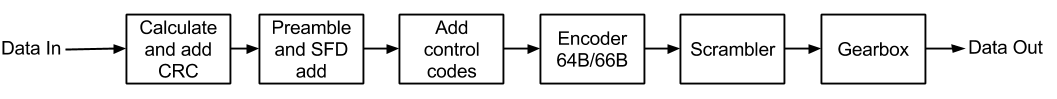
\includegraphics[scale=0.45]{EthTx}
            \caption{Ethernet Transmit}
            \label{fig:EthTx}
       \end{figure}
       
       The \textit{DataIn} is from the higher layers of the protocols which have the data to be transmitted using \gls{mac} layer protocol. Physical layer protocols are out of the scope of this thesis.
       
        
       \subsubsection*{Ethernet receive}
           The Ethernet receive sequence is shown in Fig.~\ref{fig:EthRx}. \textit{DataIn } come from the physical transmission layer and \textit{Dataout} goes to the higher protocol layers.
       
            \begin{figure}[!htb]
             \centering
             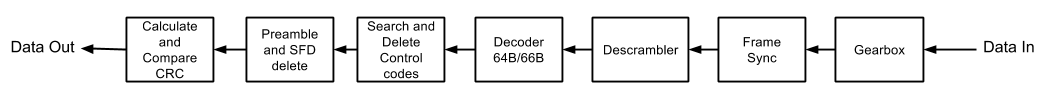
\includegraphics[scale=0.45]{EthRx}
             \caption{Ethernet Receive}
             \label{fig:EthRx}
            \end{figure}
            
       \subsubsection*{Ethernet raw frame} \label{ethrfr}
       
       The Ethernet raw frame format is represented as in Table.~\ref{ethframe}. Each of these frames enters the transmitter \textit{Datain} as in  Fig.~\ref{fig:EthTx}. It exit as \textit{ Dataout} in the receiver as shown in Fig.~\ref{fig:EthRx}. 
       
       \begin{table}[!htb]
           \centering
           
           \begin{tabular}{|c|c|c|c|c|}
               \hline
               {\bf \begin{tabular}[c]{@{}c@{}}Mac Destination\\ Address\end{tabular}} & {\bf \begin{tabular}[c]{@{}c@{}}Mac Source \\ Address\end{tabular}} & {\bf \begin{tabular}[c]{@{}c@{}}802.1Q\\ VLAN tag\end{tabular}} & {\bf Ethertype/length} & {\bf Payload} \\ \hline
               6 octets                                                                & 6 octets                                                            & 4 octets                                                        & 2 octets               & 42-1500 octet \\ \hline
            \end{tabular}
            \caption{Ethernet raw frame}
            \label{ethframe}
        \end{table}
       
       A brief functional description of each block in the transmitter and receiver section is explained below.
       
       \subsubsection*{CRC}
       
        The \gls{crc} is used to detect errors incurred during the physical transmission. The \gls{crc} value is computed by dividing the data to be transmitted with the pre-defined CRC polynomial stored in memory \cite{4066263}. The remainder of the division is known as the \gls{fcs}.\\ 
        
        On the transmitter side, the \gls{fcs} is computed for the incoming data and appended as the last 4 bytes (32bits). In the Ethernet receive, the \gls{fcs} is again computed for the incoming data and is compared with the FCS field for any errors. This block will not change the incoming data apart from appending the \gls{fcs} field.
        
        \subsubsection*{Preamble and SFD}
        The Preamble is added at the start of the frame to indicate the new Ethernet frame. This block will not change the incoming data apart from adding the Preamble (7bytes) and \gls{sfd} at the beginning of the frame (1byte).\\ 
        
        \begin{table}[!htb]
            \centering
            
            \begin{tabular}{c|l}
                \hline
                Preamble & 10101010 10101010 10101010 10101010 10101010 10101010 10101010 \\ \hline
                SFD      & 10101011                                                       \\ \hline
            \end{tabular}
            \caption{Preamble and SFD}
            \label{psfd}
        \end{table}
        
      
        In the receiver, the Preamble and SFD are identified and deleted.
        
        \subsubsection*{Control codes}
        
        The Add control codes block will add the control codes for the incoming data such that the Encoder block can use the 8 octets to encode the data based on these control codes. Idles are added to the data if the length of the data is not equal to 8 octets. Each bit in the control word represents whether the octet is data, terminate or an idle octet.
        
        
        \begin{table}[!htb]
            \centering
            
            \begin{tabular}{c|c|c|c|c|c|c|c|c}
                \hline
                {\bf Type}                                                    & Idle & Idle & Terminate & Data 4 & Data 3 & Data 2 & Data 1 & Data 0 \\ \hline
                {\bf \begin{tabular}[c]{@{}c@{}}Control \\ word\end{tabular}} & 1    & 1    & 1         & 0      & 0      & 0      & 0      & 0      \\ \hline
            \end{tabular}
            \caption{Control Word}
            \label{controlword}
        \end{table}
        
        
             
        In the receiver, the complete process is reversed. It will search for the control word and delete before forwarding to the next block.
        
         \subsubsection*{Encoder 64/66B and Decoder 66B/64B}
         
          \begin{figure}[!htb]
              \centering
              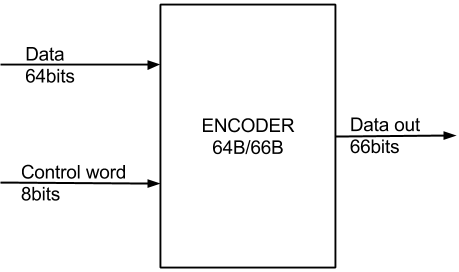
\includegraphics[scale=0.35]{encoder}
              \caption{Ethernet Encoder block}
              \label{fig:encoder}
            \end{figure}
         
         The Encoder block is represented as shown in Fig.~\ref{fig:encoder}. The 8 octet data is encoded using the control word into 66 bit output. The first 2 bits of the output are called sync header which is used for the synchronization from the receiver. The sync header \quotes{10} corresponds to data and \quotes{01} corresponds to control codes.
      
        In the decoder, the sync header is used to synchronize the 66 bits data. The process of the decoder is the reverse interpretation of the encoder module.
        
        \begin{figure}[!htb]
            \centering
            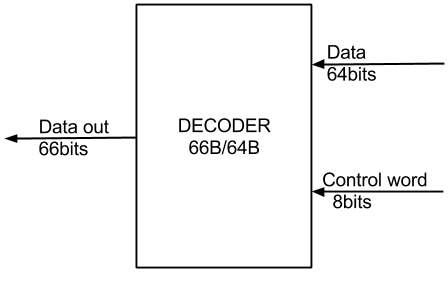
\includegraphics[scale=0.35]{decoder}
            \caption{Ethernet Decoder block}
            \label{fig:decoder}
        \end{figure}
        
        
         \subsubsection*{Scrambler and De-scrambler}
            
            This block is used to randomize the signal so that long sequences of 1's and 0's are eliminated. This is performed using the Scrambler polynomial.
            
            The De-scrambler will take the scrambled input and will output the unscrambled data.  
        
         \subsubsection*{Gearbox}

           This block is used to switch output rates. The incoming data is transmitted at different rates based on the clock frequency.
           

        
        
		\subsubsection{Xio-s}\label{xio}
		Xio-s is a Ericsson proprietary protocol used for communication between the chips.
        
        \begin{figure}[!htb]
            \centering
            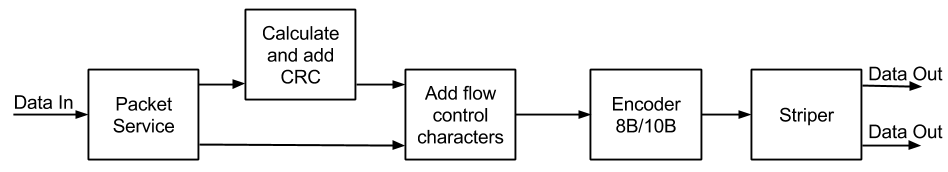
\includegraphics[scale=0.45]{Xiotx}
            \caption{Xio-s Transmitter}
            \label{fig:Xiotx}
        \end{figure}
        
        
        \begin{figure}[!htb]
            \centering
            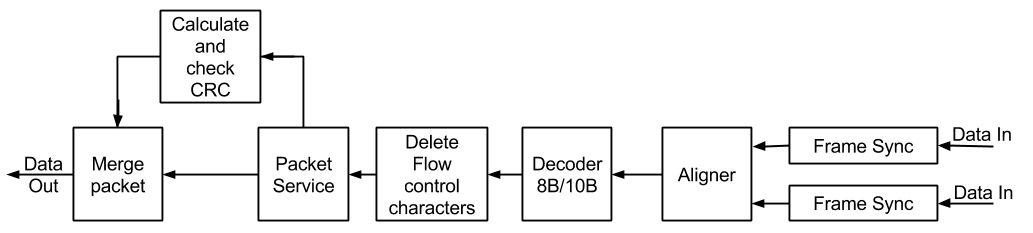
\includegraphics[scale=0.45]{XioRx}
            \caption{Xio-s Receiver}
            \label{fig:XioRx}
        \end{figure}
        
      \begin{figure}[!htb]
            \centering
            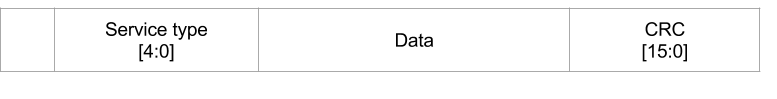
\includegraphics[scale=0.45]{xiotype1}
            \caption{Xio-s Frame format Type 1}
            \label{fig:xiotype1}
        \end{figure}
        
        \begin{figure}[!htb]
            \centering
            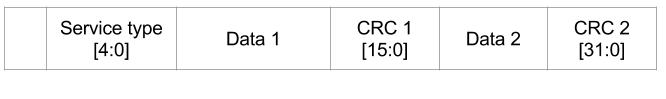
\includegraphics[scale=0.45]{xiotype2}
            \caption{Xio-s Frame format Type 2}
            \label{fig:xiotype2}
        \end{figure}
        
        There are seven different types of packet services for Xio-s protocol. These assign the packet to the proper channel based on the service type. As an example, if the service type is format 1, then it uses only CRC16 channel. Or if the service type is format II, then it uses both CRC16 and CRC32 channels.
        
        
        \subsubsection*{CRC}
        There are 16bit and 32bit CRC calculations required in the Xio-s protocol. So the polynomials for CRC16 and CRC32 are stored in memory, and the function is used according to the service type.
        
        In the receiver, the CRC is again computed and compared with the received bytes. 
        
        
        \subsubsection*{Flow control characters}
        
        The flow control character will add the control word similar to Ethernet protocol in each channel. These are used for indication of start and end of frames.
        
        In the receiver the flow and control characters are identified and deleted.
        
        
        \subsubsection*{Encoder/Decoder}
        The encoder module will encode one octet at a time to 10bits. So for 8 octect, it outputs 80bits. The encoder 8B/10B is invented by IBM and famous for short run length and DC balance.
        
        The decoder module does the reverse of the encoder and thus the output of decoder will be the same as the input of encoder.
        
        \subsubsection*{Striper}
        It is used to split the 80bits of incoming data into 40bits of two physical channels to increase the data transfer rate.
        
        
        \subsubsection*{Frame sync}
        The objective of the frame synchronization is to detect the beginning of new valid data. After the sync header is found the frame sync module outputs 66 bit blocks in the same rate as it gets the incoming blocks, the difference is that the outgoing blocks are skewed according to the placement of the sync header so that the outgoing block starts with the two bit sync header. The frame sync module will not change the incoming data, it will just adjust the boundaries of the data so that its outgoing data comes with the sync header first.
        
        
        \subsubsection*{Aligner}
        This block is used in the receiver if striper is used in the transmitter side. It aligns the two incoming 40bits channels into one 80bits channel.
        
        
		\subsubsection{CPRI}
        
         \begin{figure}[!htb]
             \centering
             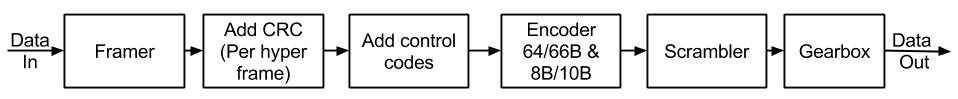
\includegraphics[scale=0.45]{cpritx}
             \caption{CPRI Transmitter}
             \label{fig:cpritx}
            \end{figure}
            
         \acs{cpri} is an industry co-operation aimed at defining a publicly available specification for the key internal interface of radio base stations between Radio Equipment Control (REC) and the Radio Equipment (RE) \cite{cpri}. It is the co-operating work of Ericsson AB, Huawei Technologies Co.Ltd, NEC corporation, Nortel Networks SA and Siemens AG.   
         All the blocks in this protocol are similar to the blocks in the Ethernet protocol. The frame structure is similar to the Xio-s protocol.
         
            
            
        \begin{figure}[!htb]
            \centering
            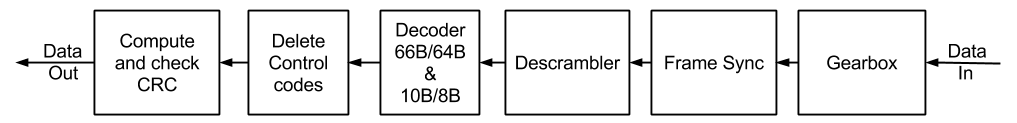
\includegraphics[scale=0.45]{cprirx}
            \caption{CPRI Receiver}
            \label{fig:cprirx}
        \end{figure}
        
		\clearpage


       \section{Modeling concepts}
        \vspace{1cm}
        \thispagestyle{plain}
      
      This chapter  explains in detail about the languages used for system level modeling. It is followed by the methodology used to verify the system.  Why and how a new language is developed for programming the architecture at Ericsson AB is explained in the section thereafter. The next section explains the meaning of grammar and language and its terms. It is further followed by the introduction of parser generator tool called Antlr.   
      
      \subsection{Introduction}
            The hardware architecture and its interconnections need to be understood to design the protocol processor. The reconfigurable architecture developed at Ericsson AB is called Freyja architecture. The hardware architecture details have to be abstracted in order to be defined in a high level description. Similarly, the Protocols details have to be represented using the same description to reconfigure the hardware for different protocols. Mapping between them requires a custom set of configuration data to define and reconfigure the architecture according to the requirement. To accomplish this, the task involves the following major steps:
            
            \begin{itemize}
                \item{Study the Reconfigurable hardware architecture.}
                \item{Identify the common protocol functions.}
                \item{Develop a grammar to describe the details in high level language.}
                \item{Test the developed system.}
               \end{itemize} 
       
      
        To study the reconfigurable hardware architecture developed at Ericsson AB, one has to understand the modeling language and the reason for its usage. So the next section will provide details about the different system level modeling languages and their abstraction details.  
      
      
      	\subsection{System-level modeling}
          
          A hardware system requires modeling concepts that allow designers to explore different aspects of the system. These concepts include communication, time, structure, hierarchy etc. As depicted in Fig.~\ref{fig:Gajski}, there are different levels of abstraction and domains in which the development phases vary. For example, in software, designers carry out performance exploration to identify bottlenecks with respect to time, excluding the lower level hardware details. The Y chart maps the different modeling styles of hardware as 3 different domains. In order to represent the hardware in these domains at different abstraction levels, an executable model is required. The designer should be able to model the different aspects of hardware, it should be scalable, possible to simulate, test and verify the functions. The Register transfer level description of the hardware is synthesized into a gate level netlist by logic synthesis tools. This level of hardware abstraction describes the signal transition between synchronously clocked registers. Traditional modeling languages have emphasized the hardware design flow, whereas the recent languages have incorporated concepts for efficient modeling at system level. With traditional languages like VHDL/Verilog, which are more used for RTL level, it takes too much time to develop for architectural exploration and software development. They also have poor performance i.e takes more time to simulate complex systems and are not available early in the development phase. In this section, Transaction Level Modeling (TLM) is introduced which is an alternative to traditional approaches for efficient abstraction and exploration of architectural details. Transaction level modeling is supported in languages such as SystemC and SpecC by abstract channels that connect communicating modules.
          
          
          \subsubsection{Language comparison}
          
          Several languages have emerged to address various aspects of system design. Fig.~\ref{fig:languagec} illustrates the comparison of different languages. Although Ada and Java have proven their value, C/C++ is predominately used today for embedded system software. The Hardware description languages, VHDL and Verilog,  are used for simulating and synthesizing digital circuits. With the increase in design complexity, with multi million gates being fabricated, the increase in pressure to get design out faster with first time design success is also higher. Many new languages are used in industries which help in designing the higher abstraction models of hardware to be used for function verification and software validation. Systemverilog helped the designer with more constructs compared to Verilog, which addresses many hardware-oriented system design issues.\\       
          
          
          \begin{figure}[!htb]
              \centering
              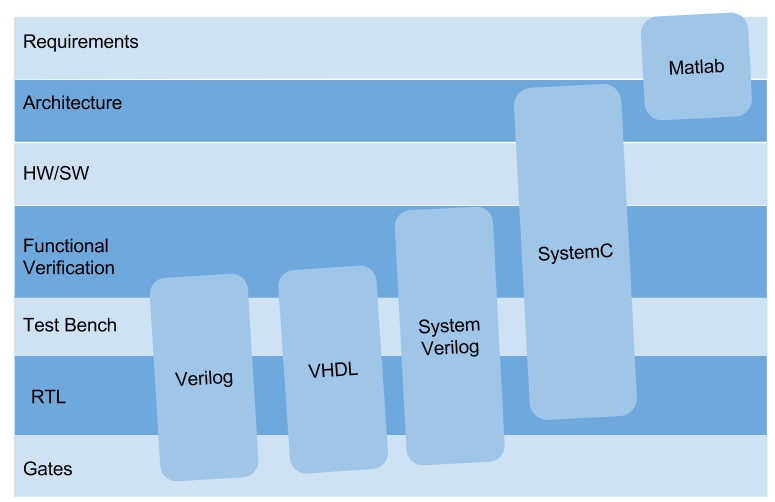
\includegraphics[scale=0.5]{languagec}
              \caption{Hardware description languages and abstraction levels \cite{groundup}}
              \label{fig:languagec}
            \end{figure}
            
            SystemC is an ANSI standard C++ class library for system and hardware design, for use by designers and architects who need to address complex systems that are hybrid between hardware and software \cite{1617814}. SystemC provides an event-driven simulation kernel in C++, together with signals, events, and synchronization primitives, deliberately mimicking the hardware description languages VHDL and Verilog. Matlab and several other tools are widely used for capturing system requirements and developing signal processing algorithms. 
            
            \subsubsection{Transaction Level Modeling}
            
            Transaction level models use abstract channels to model communication between concurrent processes in the system using function calls \cite{tlm}. In RT level each bit is instantiated as a port and hence in TLM level it can be abstracted to a byte, word or according to the architecture requirement. Also, the signal assignments of individual bits in RT level are abstracted with function calls which either send or receive the transaction. A transaction can be defined as an exchange of information between the processes in the simulation. It may contain complex data structures with control and data information, burst of data or a simple word of data packet. Time within TLM components are modeled as untimed, approximately or cycle accurate \cite{ARM:07}.\\
            
            TLM complements RT-level modeling, in order to perform following activities \cite{groundup} :
            
            \begin{itemize}
                \item{Hardware micro-architecture exploration and starting point for more detailed hardware modeling.} 
                
                \item{System level architectural exploration, such as selecting communication and processing components and Hardware/Software partitioning.} 
                
                \item{Virtual platform for software development.}
                
                \item{Reference model for hardware functional verification.}
            \end{itemize}
            
            Transaction level modeling is supported by languages like SystemC and SpecC. The communicating modules which are either initiators or targets are connected through channels. An initiator will start sending the transaction while the target will respond to the initiator request. Arbitration and routing algorithms are necessary for multiple initiators and targets to communicate in the system. The arbitration algorithm selects the initiator to be given access to the channel, and the routing algorithm assures that the correct target is addressed by transaction information. All these concepts are used to model the interconnects found in \gls{socs}. 
            
            
            \subsubsection{SystemC}
            
            SystemC is a system design language that has evolved in response to a pervasive need for a language that improves overall productivity for designers of electronic systems \cite{groundup}. The open SystemC initiative (OSCI) formed in 1999, maintained a simulation library for SystemC. In December 5 2011, Accellera Systems initiative was formed by the merger of Accellera and the Open SystemC Initiative. SystemC is a C++ library that contains routines and macros to simulate concurrent processes using HDL like semantic. SystemC is now the IEEE Std. 1666 for system-level modeling, design and verification. It offers real productivity gains for the designer by providing hardware and software components design in parallel, but at a high level of abstraction. This higher level of abstraction gives the design team a fundamental understanding of the intricacies and interactions of the entire system, early in the design process and enables better system trade offs, earlier verification, and overall productivity gains through reuse of early system models as executable specifications \cite{groundup}.\\
            
            \begin{figure}[!htb]
                \centering
                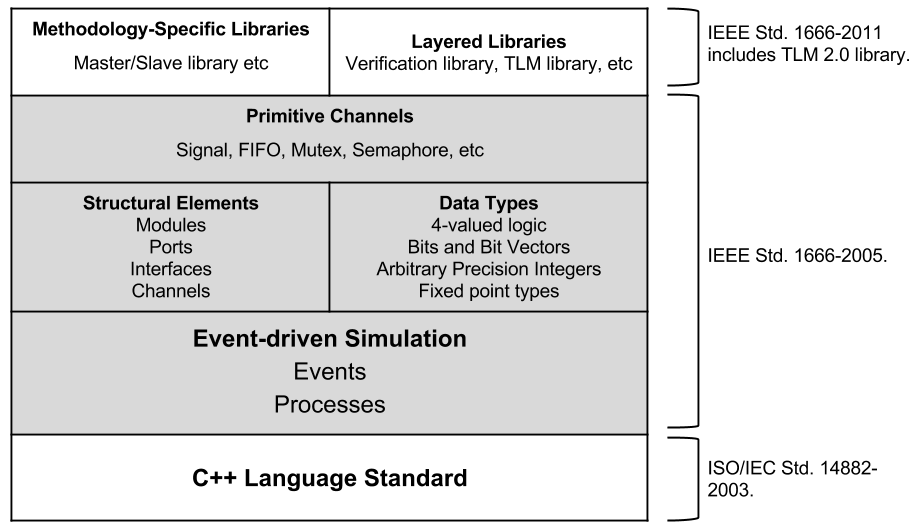
\includegraphics[scale=0.5]{Systemc}
                \caption{Layered SystemC Architecture}
                \label{fig:Systemc}
            \end{figure}
            
            
            
            Fig.~\ref{fig:Systemc} illustrates the layered architecture of SystemC. The shaded blocks are the SystemC core language standard, build upon standard C++. The layers above the standards are additional libraries available for system-level design and verification. A SystemC module encapsulates processes, which describe behavior, and communicates through ports and channels with other SystemC modules. Processes are used to describe concurrency and wait-statements are used to halt process execution for a specific time or until an event occurs. The OSCI SystemC TLM library contains ports, interfaces, channels, and also data structures are used to represent the request and response in an initiator-to-target communication scenario. The C++ notion of header (.h file) is used for the entity and the notion of implementation (.cpp file) for the architecture. Hardware by nature is concurrent and modeling it through simulation on a host processor is an illusion. It is accomplished by simulating each concurrent unit (defined as SC\_METHOD, SC\_THREAD or SC\_CTHREAD). Each unit is allowed to execute until the simulation of the other unit is required. The simulation of concurrency is the same for SystemC, Verilog, VHDL or any other hardware description languages. The simulator kernel will handle these tasks. \\
            
            In TLM2.0, an \textit{initiator} is a module that initiates the transaction and a \textit{target} is a module that responds to transaction initiated by other module. The same module can act as an initiator and as a target for example in the case of modeling a bus or a router. TLM2.0 uses sockets to send/receive transaction.\\ 
            
            
            \begin{figure}[!htb]
                \centering
                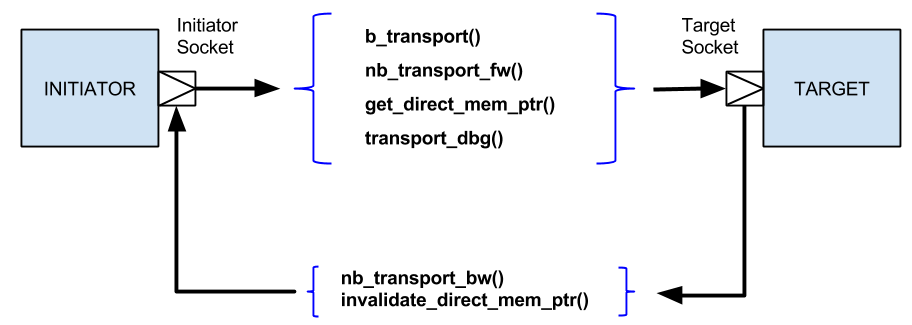
\includegraphics[scale=0.5]{sockets}
                \caption{Initiator and Target sockets}
                \label{fig:sockets}
            \end{figure}
            
            An interconnect is a component which does not modify the transaction, but merely forwards the transaction.  Fig.~\ref{fig:sockets} illustrates the different ways of function calls for data exchange through transaction. The TLM2.0 library utils provide the simple initiator and the simple target sockets for user convenience. These are used in modeling the reconfigurable architecture discussed in a further section together with sockets which allow transactions to be sent to multiple destinations.\\\\
            
            \begin{figure}[!htb]
                \centering
                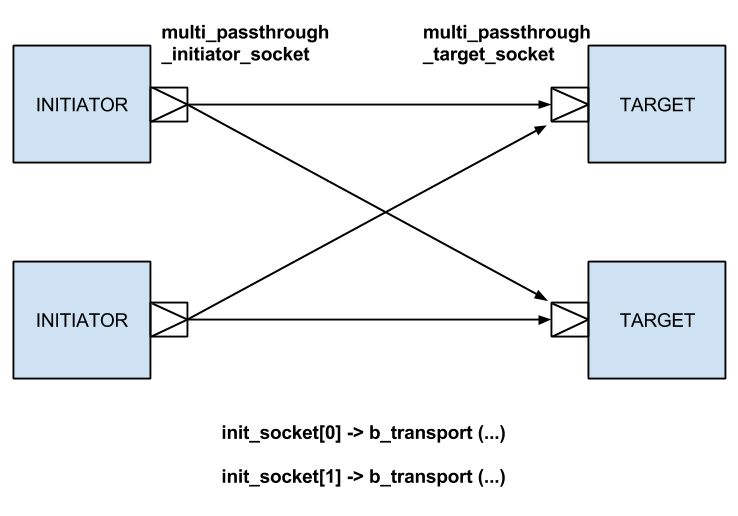
\includegraphics[scale=0.45]{multisocket}
                \caption{Many to many binding}
                \label{fig:multisocket}
            \end{figure}
            
            The transaction being routed can be represented by a simple data structure provided by TLM2.0 utils referred to Generic payload. It has a standard set of bus attributes like command, address, data, byte enables, streaming width, and response status. The command can be either write or read, the data attribute points to a data buffer within the initiator and the data length attribute will give the length of the data array. The streaming width attribute specifies the width of a streaming burst where the address repeats itself. This Generic payload is modeled in each of the reconfigurable operator blocks for initiating the transaction and the attributes are handled accordingly.    
            
            
            \subsection{Verification methodology}
            
             In the early days, digital designs were verified by looking at waveforms and performing manual checks. This is a very tedious and time consuming task for the present day complex systems. So automating the verification process using better and efficient frameworks is always preferred. The SystemVerilog language came to aid many verification engineers. Its features like classes, covergroups and constraints have helped verifying complex digital systems. Later Verification Methodologies started to appear. \gls{uvm} is one of the methodologies that was created for the need to automate verification. \gls{uvm} is a verification methodology based on the best features of \gls{ovm} and \gls{vmm} \cite{uvm}.\\
            
            
            \begin{figure}[!htb]
                \centering
                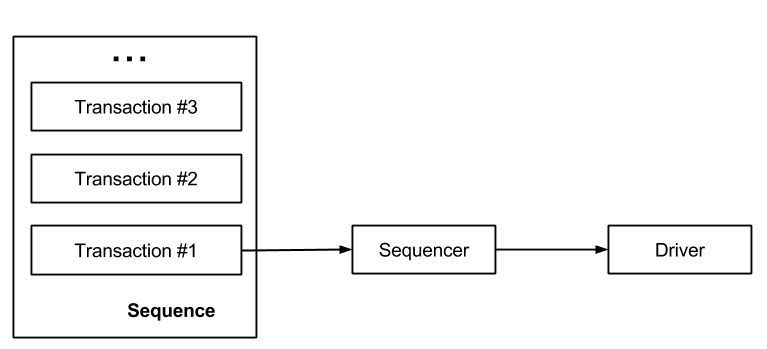
\includegraphics[scale=0.45]{sequencer}
                \caption{UVM Sequencer}
                \label{fig:sequencer}
            \end{figure}
            
            
            The first step in verifying the designed system is by defining what kind of data is to be sent to the design under test. The detailed architecture of UVM is not discussed as it is out of the thesis scope. Only features relevant to the work are summarized. A transaction can be built from uvm\_transaction or uvm\_sequence\_item classes similar to the transaction in SystemC. The "random" keyword is used to generate a transaction according to the constraints. The sequencer is responsible for sending the transaction to the driver component, which in turn connects to the Design Under Test (DUT).
            
      %\clearpage
       
       \subsection{High level description of the protocol}
          
          In general, how the reconfigurable architectures are programmed and the related work in this field is discussed in Section \ref{cgr}, wherein it explained different tools and frameworks developed for computationally intensive \gls{dsp} architectures. As coarse grain architectures are targeted for specific domains to optimize the architecture design, the synthesis tools designed for protocol processing are discussed in the next section.  
          
          
          \subsubsection{Related work}
                    
          As discussed in the previous section, SystemC enables the specification of hierarchically structured communication protocols using the concepts of interfaces and channels. The SystemC \textsuperscript{sv} \cite{1012696} discusses the way to model the complete protocol environment by  extending the SystemC language. It allows specifying the protocol  which generates the controller for producer and consumer and sends the data through abstract channels. The tool is called COSYNE (Controller Synthesis Environment).\\
          
          Clairvoyant \cite{285744} describes the protocols using a grammar based specification. It will generate an FSM described in VHDL which can be used by the logic synthesis tools. It was further commercialized and extended as the Synopsys Protocol compiler.\\
                  
          ProGrIL \cite{progril} is the Protocol Grammar Interface Language based on the Context free LL(1) grammar. The configuration file will contain the information about the widths and depths of various parts of the grammar processors, such as buses and memories.\\ 
          
          In the case of ProGram \cite{831438}  \cite{565871}, input specification is similar to the production based specification and the output is the VHDL code of register transfer level. It is distinct in specification description when compared to the other approaches wherein the production rules are independent of port widths. The port widths are specified as design space constraints and the synthesis tool will generate different designs with varying performance for different values of constraints.\\            
          
          All the above discussed methodologies try to develop a generic tool to map the protocol described in high level description directly to register transfer level. This includes the synthesis tools exploring design space for the optimized  hardware architecture with respect to area and performance. As discussed in Section. \ref{cgr}, for the computationally intensive DSP applications, there are tools which map the high level description into specific architectures. Many case studies related to custom coarse grain architectures have also been discussed which developed their own set of kernels, software, configuration data for programming such architectures.\\
                    
          
          The architecture being developed at Ericsson is a custom architecture which requires a programming tool to generate the reconfiguration data and program it according to user definition. The architecture is implemented in SystemC language and it requires a new tool to program the hardware for different configurations. A new high level language is developed to describe the custom architecture.\\   
         
           \subsection{Grammar and Language} \label{grammar}
           
           A Grammar is used to describe the syntax of a language, that is, all possible legal sentences or combination of words that make up the language. More formally, Grammar G describes all allowed legal sequences of strings. This is called the Language(G) of the grammar.\\
           
           The language in turn is made of sequences of elements which can be letters, numbers or special symbols. For example, in the word \quotes{KTH} the capital letters K, T, H are to be recognized and then the word needs to be formed. This is performed by the Lexer which recognizes the letter and forms the token.
           To be able to recognize words, Lexer needs some special constructs. These special constructs make-up the language that can be recognized by regular expressions. For example, the regular expression [0-9] recognizes a single letter in the range from 0 to 9. 
           
           
           \subsubsection{Parser}
           The Lexer scans the input character streams and forms the valid tokens. The Parser takes tokens as inputs and then based on the parsing rules in the grammar, decides the parsing strategy. The parser output can be used either to create an interpreter or a compiler. 
           
           
           \begin{figure}[!htb]
               \centering
               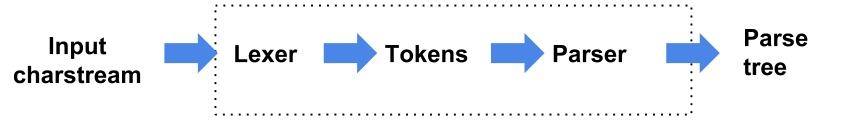
\includegraphics[scale=0.45]{parsetree}
               \caption{Parser}
               \label{fig:parsetree}
            \end{figure}
            
            
            Here, a language application is built to output the reconfigurable hardware architecture. Hence the parser output is used to translate it to the required output. 
            
            \subsubsection{Backus-Naur Form}
            
            In computer science world, \gls{bnf} is the notational technique for context free grammars. It is a set of derivation rules to define the language.\\ 
            
            For example,\\
            
            \la int\ra  \hspace{0.1cm} ::= \la DIGIT \ra    | \la int \ra  \la DIGIT \ra \\
            
            \la DIGIT \ra \hspace{0.1cm} ::= [ 0-9 ]\\
            
            In the above grammar, \la int \ra on the left hand side is called as non terminal and the \la DIGIT \ra is called as terminal. So the sequences of digits like 9999... can be parsed by representing the grammar according to the above \gls{bnf} code. 
            An extension to BNF grammar with more operators to write the syntax is called as EBNF. The grammar above can be rewritten in EBNF as below \\
            
            \la int \ra \hspace{0.1cm} ::= \la DIGIT \ra + \\
            
            Here \quotes{+} means one or more occurrences of digits. Similarly \quotes{*} operator means 0 or more occurrences.
          
          
          A high level language description requires the design of Lexer and parser from scratch. They can be designed using languages like C, C++, Java, C\# and more. Based on the application requirement, a parsing strategy needs to be decided. As the machine resources grew in today's world, researchers have developed more complex and powerful Non Deterministic parsing strategies. Today both \quotes{bottom-up} and \quotes{top-down} approaches exist. Developing a \quotes{bottom-up} parsers is hard to understand and debug, compared to the \quotes{top-down} parsers.\\
          
          There are many tools like Antlr4, APG, AXE, YACC etc which help to build a language application. They provide the user with Lexer and Parser implementations for the grammar defined by the user. This helps in building the language application in a short time. Antlr is one such tool which helps in designing a recursive descent top-down parser with a clear error recovery mechanism.           
         
         \subsubsection{Antlr}
             
            Antlr4 accepts as input any context-free grammar that does not contain indirect or hidden left-recursion \cite{antlr4}. Antlr4 generates a recursive descent top down parser.  Antlr4 parser uses a new parsing technology called Adaptive LL(*). ALL(*) prediction mechanism launches sub parsers at decision points and they operate in pseudo parallel to explore all possibilities of input combinations. It performs the grammar analysis dynamically at runtime rather than statically. Antlr4 currently generates parsers in Java or C\#, and the previous version supports even C and C++.\\ 
            
            
              \begin{figure}[!htb]
                  \centering
                  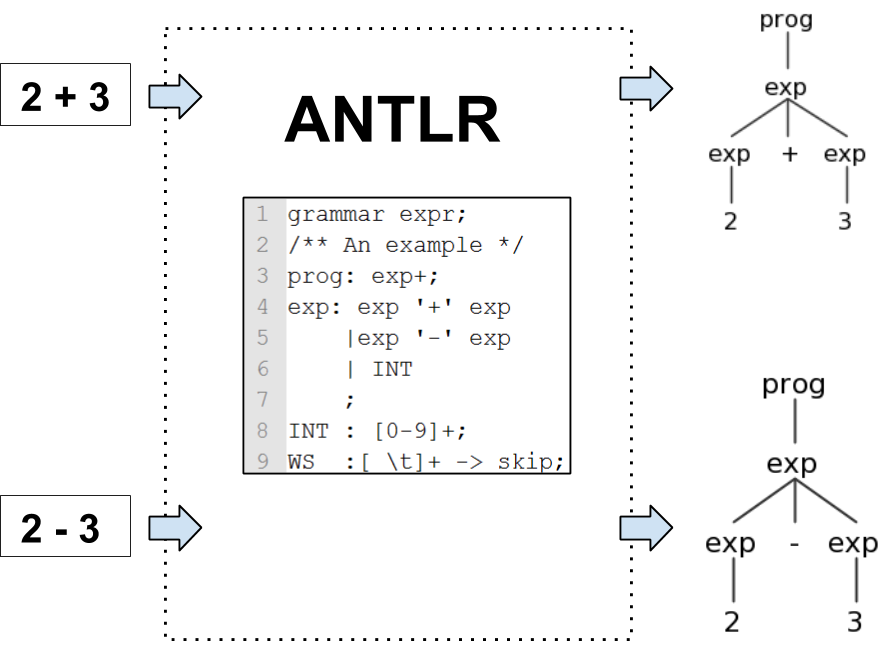
\includegraphics[scale=0.4]{antlr}
                  \caption{Antlr : Input, Grammar and Parsetree}
                  \label{fig:antlr}
                \end{figure}
            
            Antlr4 grammar uses Yacc-like syntax with EBNF operators like the Kleene star(*) and token literals in single quotes. Both lexical and syntactic rules are specified in the same grammar file. The Lexical rules are specified in capital letters which distinguishes them from others.\\
            
            
            Fig~\ref{fig:antlr} illustrates Antlr's Yacc-like metalanguage. Antlr4 automatically rewrites the rules to be non left recursive and unambiguous. The grammar analysis is performed dynamically and results are cached in lookahead Deterministic Finite Automaton (DFA) for efficiency \cite{antlr4}. 
             
          
             \subsubsection*{Parse tree listeners and visitors}
             Antlr provides two tree walking mechanisms in its runtime library. In parse tree Listeners, Antlr generates a ParseTreeListener subclass specific to each grammar with entry and exit methods for each rule. This is suitable for applications wherein the complete tree needs to be invoked from root until the last leaf node in-order. This is the default method in Antlr. The advantage of using ParsetreeListener mechanism is that it generates automatic \gls{apis} for the walker sequence and it is easier to build the language application.\\ 
             
             
             In many circumstances, the designer needs to control the walk sequence. It is not possible to design a language application with visitor method which generate \gls{apis} from the left to the right leaf node. The parse tree visitor mechanism is used when the tree walking needs to be controlled. Option -visitor makes Antlr4 to generate a visitor interface from a grammar with a visit method per rule. Then in the application-specific code, a visitor implementation can be called.\\
        
        \clearpage
        

		\section{Freyja architecture}
        \vspace{1cm}
        \thispagestyle{plain}
            
         The three protocols discussed in the background are compared to highlight the common functions shared between them. The reconfigurable architecture called Freyja is explained in detail in the next section, and then a language description is developed to define the Freyja architecture which maps different protocol operators and their interconnections. The high level description accounts for different operator instantiation, transaction routing, constants in memory and error handling. Each of these is explained in detail in this chapter.
            
            
        \subsection{Comparison of the protocols} \label{protocol}
        
        The parser generator tools need to be used to describe the protocols and produce the reconfigurable files for the hardware architecture. The protocols of the MAC layer considered in this work are explained in section \ref*{protocols}.\\ 
        
        The common functions in each protocol are highlighted with the same color for the boundary line in Fig~\ref{fig:common_tx} \& Fig~\ref{fig:common_rx}. Each of the operators are implemented in SystemC and they receive and process the TLM2.0 transaction to perform the corresponding tasks.\\ 
        
        
        
        \begin{figure}[!htb]
            \centering
            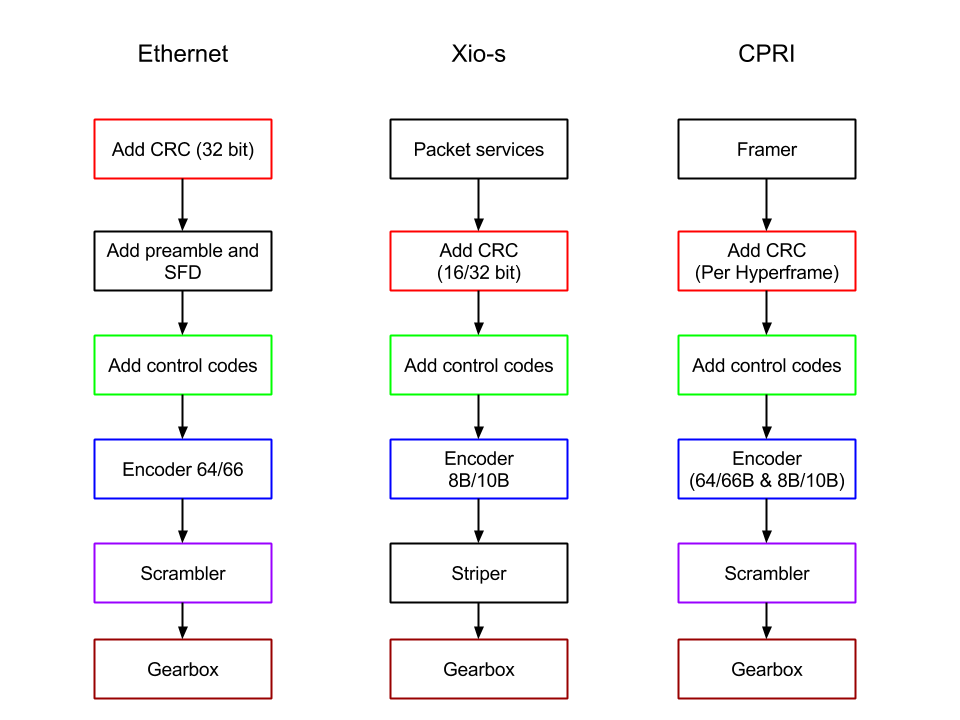
\includegraphics[width=1.1\textwidth]{common_tx}
            \caption{Transmitter of all three protocols}
            \label{fig:common_tx}
        \end{figure}
        
        
        The operators can be multiplexed and a generic operator unit can be designed for the blocks with same color boundary line. For example, the FCS computation is required in all three protocols. They require 16/32 bit polynomial to compute the checksum value. The memory unit stores the polynomials and control data required for the CRC operator to perform a CRC16 or CRC32 operation. Since the CRC check operation performed in the receiver stage, also requires the computation of FCS, a single operator unit can be designed and configured to perform different operation. The CRC operator will be designed in a way, such that it is used to transmit the received transaction by appending the FCS value, and if the transaction is from receiver stage, then the same hardware is used to compute the checksum value and then compared with the received checksum value. The operator switches its context based on the control information received form the memory block. A common hardware architecture can be designed with minimal reconfiguration to perform the protocol processing of different protocols mentioned above.\\
        
        
        
        \begin{figure}[!htb]
            \centering
            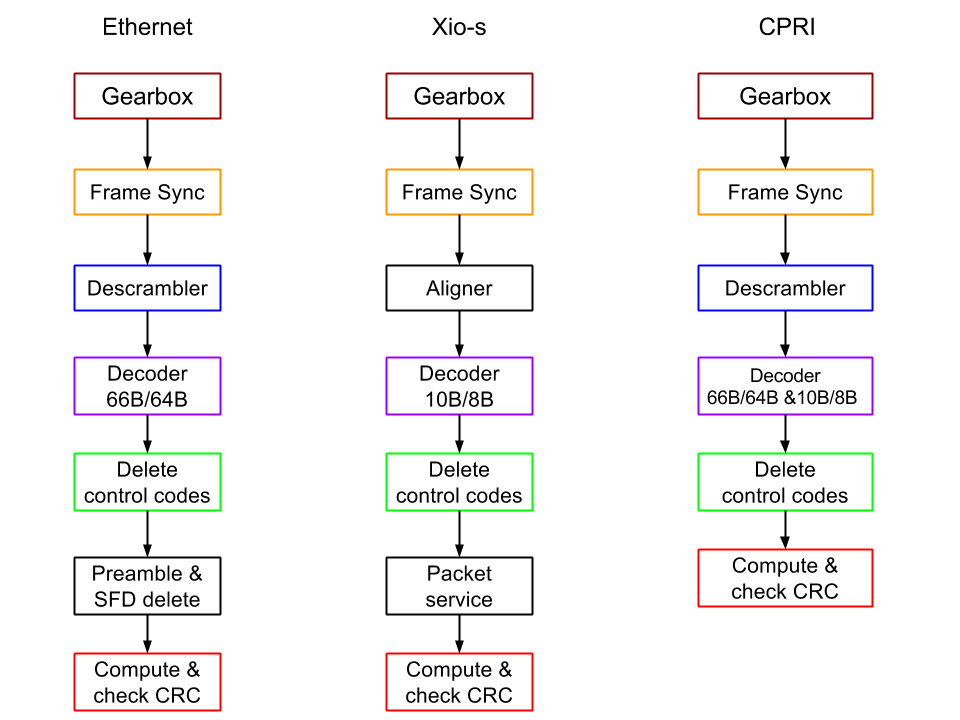
\includegraphics[width=1.1\textwidth]{common_rx}
            \caption{Receiver of all three protocols}
            \label{fig:common_rx}
        \end{figure}
       
             
       \subsection{Architecture details} \label{freyja}
       
       As depicted in Fig~\ref{fig:Freyja}, Freyja architecture is a reconfigurable protocol processor. It consists of different protocol operators which are connected through the central switch. This switch based network topology can be configured to process the data based on protocols. The Ring bus (RB) interfaces the Freyja with higher layers. It issues the tokens with data frames from different protocols. The Common Memory Interface (CMI) is used to fetch the data from memory. The physical interface is represented by the Serializer/Deserializer block i.e SERDES. The details of each of the Freyja architecture blocks are discussed below.\\
       
       \begin{figure}[!htb]
           %\centering
           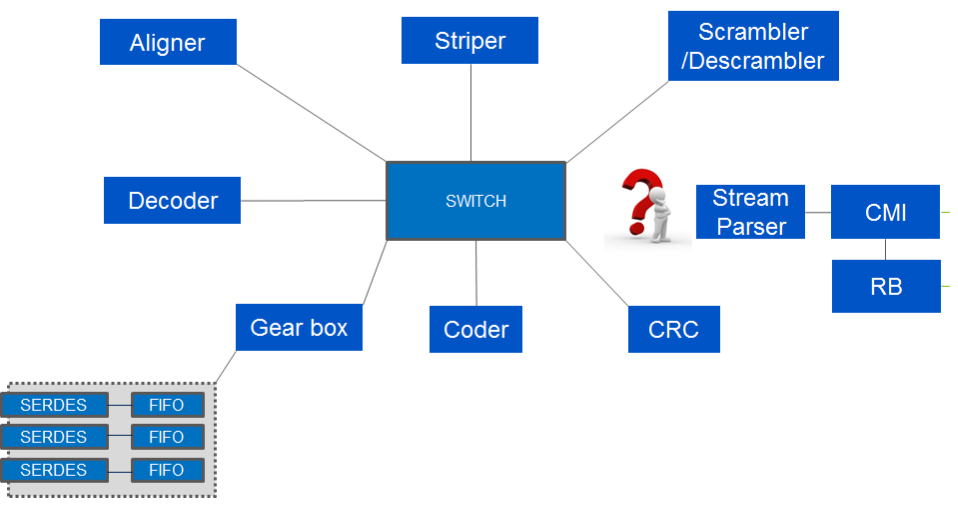
\includegraphics[width=1.1\textwidth]{Freyja}
           \caption{Switch based Freyja network topology}
           \label{fig:Freyja}
       \end{figure}
       
       %\clearpage
       \subsubsection{Switch port}
       
       \begin{wrapfigure}{R}{0.4\textwidth}
           \vspace{-30pt}
           \centering
           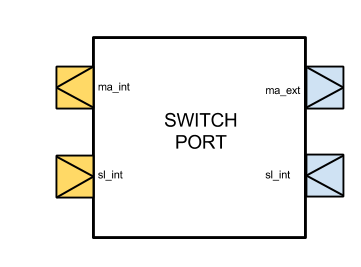
\includegraphics[width=0.4\textwidth]{switchport}
           
           \caption{Switch port}
           \label{wrap-fig:switchport}
           
       \end{wrapfigure} 
       
       Freyja switch port is the smallest unit in the architecture. It receives the transaction from different functions and then forwards it to the internally connected next switch port based on the destination address of the transaction. It consists of a \textit{simple initiator socket}, a \textit{simple target socket}, a \textit{multi pass through initiator socket} and a \textit{multi pass through target socket}. It is illustrated in \lipsum[0-0] Fig~\ref{wrap-fig:switchport}.\\
       
       \subsubsection{Operator units}\label{operator}
       
       
       \begin{figure}[!htb]
           \centering
           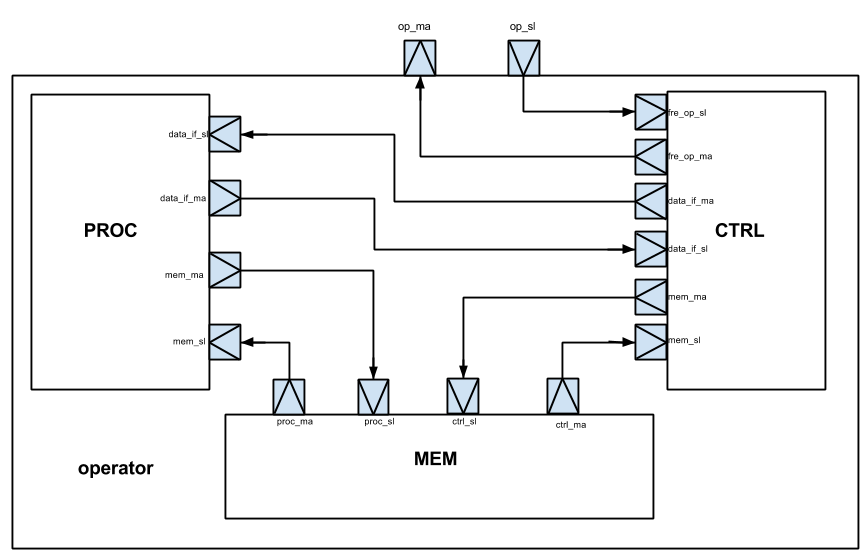
\includegraphics[scale=0.5]{operator}
           \caption{Freyja operator}
           \label{fig:operator}
       \end{figure}
       
       
       Freyja Operator units are designed to contain a control, a process and a memory block. Each operator function is implemented in the process block, and the transaction routing and context switching is performed in the control block. The memory block stores the constants required for the process block. It can also be used to store the process block results. The control block receives the result directly from process block transaction or from the memory contents. 
       
       As in Fig~\ref{fig:operator}, the three components of each operator are encapsulated with one simple initiator socket and one target socket which initiates and receives the transaction from the switch respectively. The transaction received is routed to the control block. The control block will inform the memory block to encapsulate the required data for the particular operator and to send it to process block. Meanwhile the received transaction is sent to the process block from the control block to perform the required operation. 
       
       
       \subsubsection{Switch wrapper}
       The switch wrapper instantiates the switch ports and their interconnections. Based on the number of operators, the required number of switch ports is instantiated.
       
       
       \begin{figure}[!htb]
           \centering
           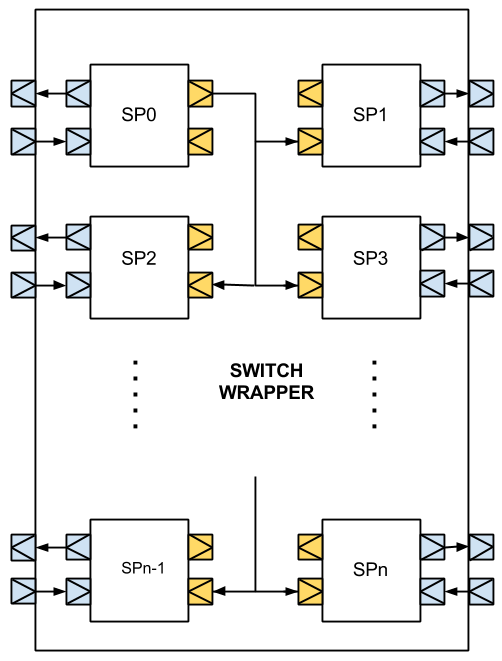
\includegraphics[scale=0.5]{switchwrapper}
           \caption{Freyja Switch Wrapper}
           \label{fig:switchwrapper}
       \end{figure}
       
       As can be seen in Fig~\ref{fig:switchwrapper}, each switch port can send the transaction to any of the other switch port through the internal multipassthrough socket. The other switch ports can receive the transaction using the multi pass through receive socket. A transaction source and destination cannot be the same operator as there is no such interconnection.
       
       \subsubsection{Overall architecture}
       
       An illustration of Freyja architecture with four operator units is shown in Fig~\ref{fig:Overallarchitecture}.
       
       
       \begin{figure}[!htb]
           \centering
           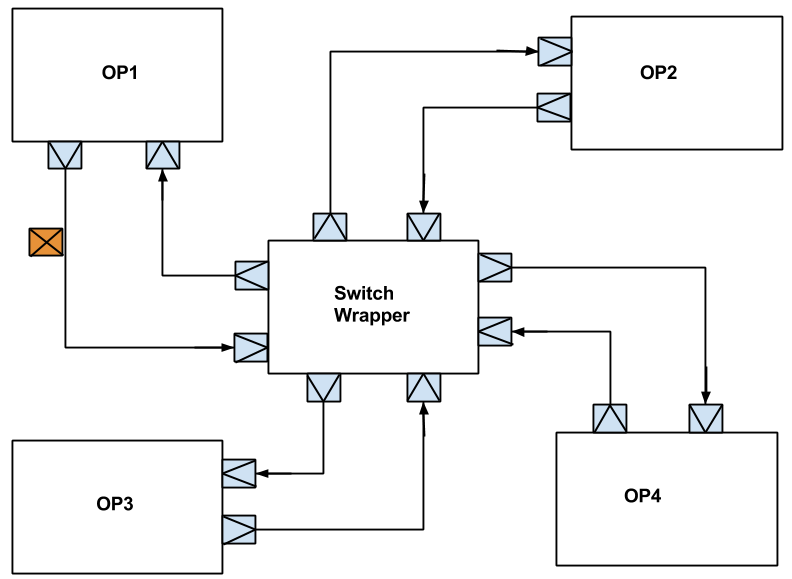
\includegraphics[scale=0.5]{Overallarchitecture}
           \caption{Freyja Architecture for 4 operators}
           \label{fig:Overallarchitecture}
       \end{figure}    
       
       The overall Frejya architecture consists of switch wrapper instantiating switch ports, and the operator blocks. A transaction originating from operator 1 as shown in Fig~\ref{fig:Overallarchitecture} with orange box can be routed to any of the other operators as destination based on the address of the payload header data. This will be assigned in the control block of the operator.   
            
        \subsection{Parser implementation}
            The Antlr tool is used as a parser generator to develop the language. The grammar is defined using EBNF.\\
            
            
             \begin{figure}[!htb]
                 \centering
                 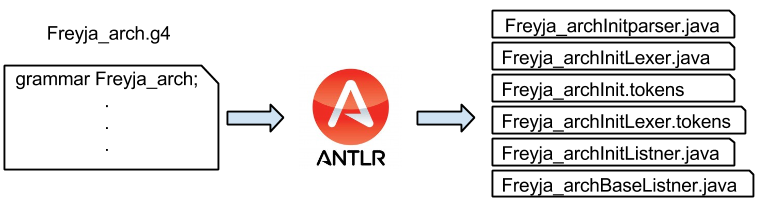
\includegraphics[scale=0.5]{antlrfiles}
                 \caption{Antlr generated Files}
                 \label{fig:antlrfiles}
                \end{figure}
        
        A brief description of the generated file is stated below:\\
        
        \textbf{Freyja\_archInitparser.java:} This file contains the parser class definition specific to the grammar in freyja\_arch.g4 (Appendix \ref{gramr}), that recognizes the syntax of Freyja protocol processor language.\\
        
        \textbf{Freyja\_archInitLexer.java:} This file contains the lexer class definition by analyzing the lexical rules in the grammar.\\
        
        \textbf{Freyja\_archInit.tokens:} Antlr generates a token type number to each token in the grammar and store these values in this file.\\
        
        \textbf{Freyja\_archInitListner.java, Freyja\_archBaseListner.java:} The Antlr parser builds a tree walker that can trigger the callback events to a listener object. Freyja\_archInitListner is the interface that describes the callbacks and Freyja\_archBaseListner is a set of empty default implementations.\\
        
        The back-end functions are implemented to produce the Freyja architecture based on the described language. 
        
        
        \subsection{Operator Instantiation}\label{opinst}
        
        As illustrated in Fig~\ref{fig:CRC}, each of the operators in the Freyja architecture consists of a control block to take care of the transaction routing and error handling, and a memory block for storing the constants and results, and the process block to perform the operator function.
        
        
         \begin{figure}[!htb]
             \centering
             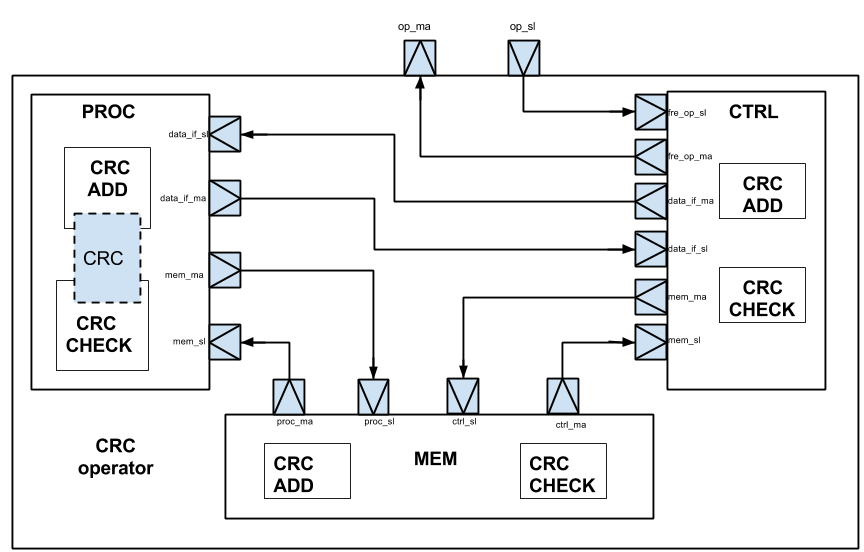
\includegraphics[scale=0.5]{CRC}
             \caption{CRC operator in Freyja Architecture}
             \label{fig:CRC}
            \end{figure}
            
            
             The functions performed during the transmitting stage might need to be performed in the receiver stage of a protocol processor.
             For instance, FCS is appended during the transmitting stage and in the receiver stage the computation of CRC is performed again. In addition, it performs the comparison of the received FCS value and the newly computed value to identify if the received data is erroneous or not.\\
 
            The control block of each operator has to identify the destination operator within the process block to forward the payload to the respective operator. The language described has to consider this feature when instantiating the operator and defining the control blocks for each operator. An example of CRC block with \textit{crc\_add} and \textit{crc\_check} operators are discussed further.\\
            
            As in Fig~\ref{fig:CRC}, the CRC computation function is used by both operators. The control block has to check if the destination operator is \textit{crc\_add} or \textit{crc\_check}, and forwards the data to be processed to the correct operator. The operator is defined as below:\\
            
            
            
            \begin{figure}[!htb]
                
            
            \begin{lstlisting}
            
<@\textcolor{blue}{Operator}@> CHECKSUM{
<@\textcolor{red}{sc\_name} @>: crc;
<@\textcolor{red}{op\_type} @>: crc_add, crc_check;
<@\textcolor{red}{op\_mem} @>: 0x01, 0x04, 0xc1, 0x1d, 0xb7, 0x20, 0x00, 0x04, 0x03, 0x04, 0x00,
           0x00, 0x01, 0x59, 0x53, 0x10, 0x03, 0x02, 0x04;
<@\textcolor{red}{errorid} @>: 02, 03;
} 
         \end{lstlisting}
         \caption{Freyja Operator Instantiation}
         \end{figure}
         
         
         \begin{itemize}
             \item{\textbf{Operator:} This is the keyword used to define the operator. \quotes{CHECKSUM} should be the unique operator name in Freyja architecture.}
             \item{\textbf{sc\_name:} This keyword is used to define the operator file name. It create the systemC files fre\_op\_ctrl\_crc, fre\_op\_proc\_crc and fre\_op\_mem\_crc which are the control, process and memory blocks, respectively.}
             \item{\textbf{op\_type:} This keyword is used to define different operators like \quotes{crc\_add} and \quotes{crc\_check} inside one \textit{Operator} block. Each operator definition also takes care of inserting a switch port and modifying the interconnections of switch wrapper function.}
             \item{\textbf{op\_mem:} This keyword is used to define the constants to be stored inside the local memory of Operator \quotes{CHECKSUM}. The constant 0x04C11DB7 stored in 1 to 4 bytes is the CRC32 polynomial, byte 5, 6 and 7 are reserved for indicating the crc control information like crc\_type, crc\_len\_conf and length\_conf. Similarly the polynomial for CRC16 and control information is stored from byte 9 to 18.}
             \item{\textbf{errorid:} This keyword is used to indicate the error id for each operator. A unique number is assigned for each of the op\_type string of all operators. In \quotes{CHECKSUM}, crc\_add and crc\_check is assigned with error id 2 and 3 respectively.}
            \end{itemize}
               
         
        
        \subsection{Context switching}
        
        The context switching in the process block is performed based on the destination operator for the data packet. The control block will determine the protocol and destination operator for the data packet. The control block will then forwards the transaction to the process block where the context switching between the operators are performed. The operator type field will indicate the process block to switch between the operators.\\
        
        As depicted in Fig~\ref{fig:CRC}, the control block determines the protocol and the operator type for the CRC operator. It then informs the memory blocks with the transaction payload to send the required information to process block. Simultaneously, the control block will send the received transaction to the process block. The memory block will send the constants required for the operator through a transaction. The process block will do the context switching of operator between \textit{crc\_add} and \textit{crc\_check} to obtain the result according to the destination operator. Once the results are obtained, the process block will send them to the control block. The control block will forward the transaction to the destination operator. 
        
      
        \subsection{Memory}
        
        The memory block is designed to store the constants required for the operators. The constants to be stored in the memory are indicated in the \textit{op\_mem} field as explained in section \ref{opinst}. Each operator is allowed to store all the constants in the memory and based on the operator in use, the constants can be forwarded to the process block through a transaction. As in the operator checksum definition, the memory contains 19 bytes which are used by the CRC16 and CRC32 operators.\\
         
         
        
        \begin{figure}[!htb]
         \label{fig:mem}   
        
         \begin{lstlisting}
<@\textcolor{blue}{memory} @>{
<@\textcolor{red}{crc\_add} @>   :00 to 08;
<@\textcolor{red}{crc\_check} @> :00 to 07, 09;
<@\textcolor{red}{scram} @>     :00 to 07: 
<@\textcolor{red}{descram} @>   :00 to 07;
} 
        \end{lstlisting}
        \caption{Freyja Memory content definition}
        \end{figure}
        
        Memory transaction for each protocol are described in the language shown in Fig~\ref{fig:mem}. The first 8 bytes of memory contents are sent as a transaction for \textit{crc\_add} operation in Ethernet protocol. The memory bytes can be written as individual bytes (for example, 01, 02, ...), or as contiguous location (for example 01 to 04, 08 to 10 ...), or a combination of both. Each protocol with the memory code as above can send transactions for different operators. In the above code, the \textit{crc add}, \textit{crc check}, \textit{scram} and \textit{descram} send the transaction to their respective blocks.
        
        
        \subsection{Transaction handling}
        
        The transaction routing for each protocol is described in the input file using the below syntax \\
        
        CONNECT: <source operator> to <Destination operator>\\
        
        Based on these all the control blocks will be configured with the destination address for the payload. The switch interconnect will send the transaction to the next operator based on this address. This mapping defines the transaction routing for each protocols and is used to build the destination address automatically using the input description. 
        
        \subsection{Error handling}
        
        Any erroneous packet can be sent to the error handler from each of the operator. The control block will verify the result and if the error flag is raised, the transaction is encoded with the corresponding error id of the operator and forwarded to the error handler. The error id for each operator  is indicated with the keyword \quotes{errorid} as explained in section \ref{opinst}.\\
        
        
		\clearpage
        
        \section{Illustrative example}
        \vspace{1cm}
        \thispagestyle{plain}
        This chapter explains the analysis of the framework through the integration of Ethernet protocol into the Freyja architecture. Ethernet operators are integrated into the system of files generated from the Antlr tool. To show the context switching between different protocols, Xio-s CRC16 operator is also integrated. The first section analyses the process and results of Ethernet integration and section \ref{xios} explains the Xio-s protocol integration.
        
        
        \subsection{Ethernet}
        
        \autoref{Ethernet} shows the complete description of Ethernet protocol. The description starts with the keyword "FunctionUnits" followed by the architecture name, followed by the description of all the operators in the Freyja protocol processor shown in Fig.~\ref{fig:Freyja}. Each of the \quotes{Operator} corresponds to the protocol functions discussed in the section \ref{ethr}.
        It is followed by the \quotes{protocol} keyword and information specific to Ethernet protocol. In the \quotes{fields} section, the raw ethernet frame is represented. This information helps in decoding the corresponding data for debugging purpose only. The \quotes{memory} section described the constants in the local memory blocks. For Ethernet protocol, the \textit{crc\_add},  \textit{crc\_check}, \textit{scram} and \textit{descram} process block will receive the constants from the memory block located in each of their Operator block.\\ 
        
        The operators involved in Ethernet transmit and receive sequence were shown in Fig.~\ref{fig:EthTx} and Fig.~\ref{fig:EthRx}, but are reproduced below in Fig.~\ref{fig:ethernet}. The \textit{Datain} in the transmit is passed from the UVM test bench. A UVM sequence is generated with the first byte indicating the protocol and the second byte containing the address of the \quotes{PROCESSOR} operator. Once the transaction reaches the \textit{switch wrapper}, it is decoded and forwarded to the \textit{proc\_tx} operator. The \textit{proc\_tx} operator is defined to extract the data from transaction payload.\\

      
         Implemented in our high level language, the interconnection between different Ethernet operators is explained in this section. A part of the Ethernet transmitter description is shown in Fig.~\ref{fig:ethh} and the receiver description is shown in in Fig.~\ref{fig:ethrr}. The corresponding interconnection in Freyja (switch wrapper interconnection is not shown) for the Ethernet protocol is shown in Fig.~\ref{fig:ethernet}.\\\\\\
        
        \begin{figure}[!htb]
            \label{fig:ethh}
            
            \begin{lstlisting}
            <@\textcolor{blue}{Tx\_PATH} @>{
            <@\textcolor{red}{CONNECT} @>: proc_tx <@\textcolor{red}{to} @> crc_add; 
            <@\textcolor{red}{CONNECT} @>: crc_add <@\textcolor{red}{to} @> pre_sfd_add;
            <@\textcolor{red}{CONNECT} @>: pre_sfd_add <@\textcolor{red}{to} @> cc_a;
            <@\textcolor{red}{CONNECT} @>: cc_a <@\textcolor{red}{to} @> enc;
            <@\textcolor{red}{CONNECT} @>: enc <@\textcolor{red}{to} @> scram;
            <@\textcolor{red}{CONNECT} @>: scram <@\textcolor{red}{to} @> gb_tx;
            <@\textcolor{red}{CONNECT} @>: gb_tx <@\textcolor{red}{to} @> gb_rx;
            }       
            
            \end{lstlisting}
            \caption{Ethernet transmitter description}
            \medskip
        \end{figure}  
        
        
         \begin{figure}[!htb]
             \centering
             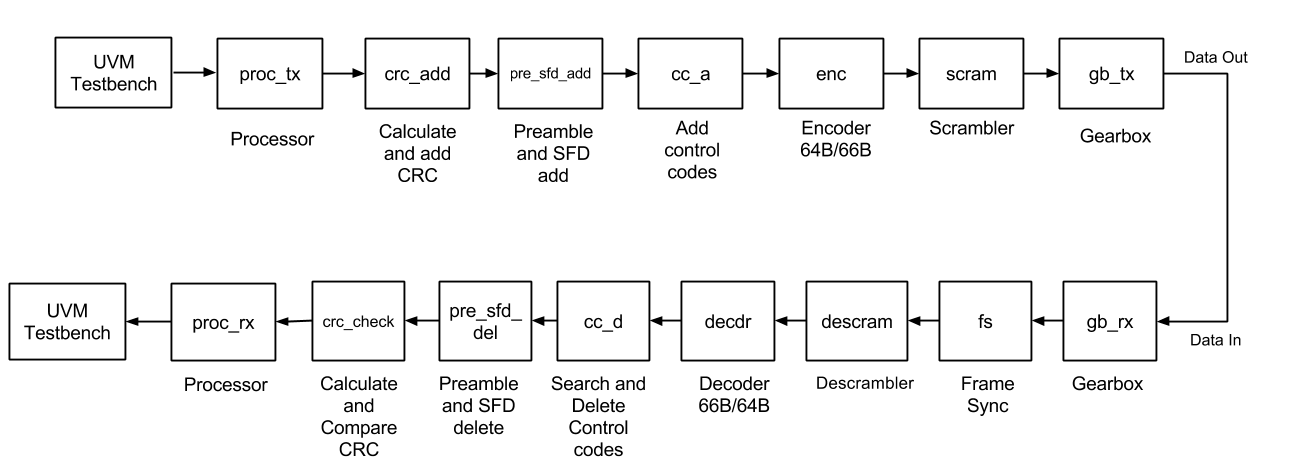
\includegraphics[scale=0.4]{ethernet}
             \caption{Ethernet protocol interconnection in Freyja}
             \label{fig:ethernet}
             \smallskip
            \end{figure}
            
        
        
        
        \begin{figure}[!htb]
            \label{fig:ethrr}
            \begin{lstlisting}
<@\textcolor{blue}{RX\_PATH} @>{
<@\textcolor{red}{CONNECT} @>: gb_rx <@\textcolor{red}{to} @> fs;
<@\textcolor{red}{CONNECT} @>: fs <@\textcolor{red}{to} @> descram;
<@\textcolor{red}{CONNECT} @>: descram <@\textcolor{red}{to} @> decdr;
<@\textcolor{red}{CONNECT} @>: decdr <@\textcolor{red}{to} @> cc_d;
<@\textcolor{red}{CONNECT} @>: cc_d <@\textcolor{red}{to} @> pre_sfd_del;
<@\textcolor{red}{CONNECT} @>: pre_sfd_del <@\textcolor{red}{to} @> crc_check;
<@\textcolor{red}{CONNECT} @>: crc_check <@\textcolor{red}{to} @> proc_rx;
}
\end{lstlisting}
         \caption{Ethernet receive description}
         \medskip
        \end{figure}  
    
    
        \vspace{5cm}
        The operators required by the protocols are first instantiated by defining them in the description. The string \quotes{protocol} indicates the definition of new protocol in Freyja architecture. It consists of 3 segments : \textit{Fields}, \textit{Tx\_path}, \textit{Rx\_Path}. 
        \begin{itemize}
            
            \item{The \textit{Fields} section is defined to indicate the details of the transaction contents in each protocol.}
            \item{\textit{Tx\_Path} is used to define the transmitter sequence.}
            \item{\textit{Rx\_Path} is used to define the receiver sequence.}
            
        \end{itemize}
        
        The \textit{Tx\_Path} and \textit{Rx\_Path} are for the user to distinguish between the transmitter and receiver sequence for each protocol. In the Freyja architecture, the interconnections have no difference with respect to the \textit{Tx\_Path} and \textit{Rx\_Path}. The interconnect information is used to code the control block of each operator to forward the transaction to the correct destination. The Antlr output for Ethernet protocol with \textit{crc\_add} and \textit{crc\_check} operator in \quotes{CHECKSUM} operator is shown in Fig~\ref{fig:ctrlblk}.
        
        \begin{figure}[!htb]
         \label{fig:ctrlblk}   
            \begin{lstlisting}
            //part of fre_op_ctrl_crc.cpp block 
            
            if(type == ethernet){
                if(op_type == crc_add){
                    data[0] = ethernet;
                    sz = sz + 2;
                    data[1] = pre_sfd_add;
                    gp.set_address(crc_add_2_pre_sfd_add);
                }
                else if(op_type == crc_check){
                    data[0] = ethernet;
                    sz = sz + 2;
                    data[1] = proc;
                    gp.set_address(crc_check_2_proc);
                }             
            }    
            \end{lstlisting}
            \caption{Freyja CRC operator Control Block code segment.} 
        \end{figure}
        
        In the above code, the CRC operator's control block initially checks for the protocol and then for the type of the operator. As illustrated in Fig.~\ref{fig:CRC}, the CRC operator multiplexes two operations. The \textit{crc\_add} and \textit{crc\_check} operators share the control block, the common memory and, hardware for CRC computation. The \textit{crc\_add} need extra logic to append FCS value to the data payload and \textit{crc\_check} requires extra logic to compare the computed and received FCS value.\\ 
        
        Based on the input description, Antlr will generate the reconfiguration data. The destination address of the transaction is configured using this data. This information is compiled in the form of constants in the SystemC environment. The language supports the possibility to send the transaction to different operators from the same source.\\ 
        
        \begin{figure}[!htb]
            
            
            \begin{lstlisting}
            // output file : fre_constants.h
            //constants for the protocol : ethernet
            const unsigned char ethernet = 0;
            const  int proc_2_crc_add=0;
            const  int crc_add_2_pre_sfd_add=1;
            const  int pre_sfd_add_2_cc_a=2;
            const  int cc_a_2_enc=3;
            const  int enc_2_scram=4;
            const  int scram_2_gb=5;
            const  int gb_2_descram=5;
            const  int descram_2_dec=7;
            const  int dec_2_cc_d=8;
            const  int cc_d_2_pre_sfd_del=2;
            const  int pre_sfd_del_2_crc_check=1;
            const  int crc_check_2_proc=0;             
            \end{lstlisting}
            \caption{Freyja Reconfiguration constants.} 
        \end{figure}
        
        The constants are formed using a simple syntax as below \\
        
        \la source operator \ra \_2\_ \la Destination operator \ra \\
        
        The constant value assigned is calculated by the parser based on the switch port interconnections. The CRC operator also contains 19 bytes of memory elements. These 19 bytes are used by both CRC32 and CRC16 Operators. The Ethernet protocol uses only CRC32 and hence only \textit{crc\_add} and \textit{crc\_check} uses the first 9 bytes of the memory elements. After the control block informs the memory about the protocol and operator, the memory block will send the transaction to the process block which includes the constants required by the operator.   
        
        
        \subsection{Xio-s}\label{xios}
        
        The Xio-s protocol is briefly explained in section \ref{xio}. The CRC block of Xio-s protocol is integrated into the system. The control block will check for the type of protocol, prioritized according to the description in the input file. Similarly, the Operators are prioritized in the order they have been defined in the input file. Defining Xio-s after the Ethernet protocol description will change the control block code segment as shown in Fig.~\ref{fig:enxios} .\\ 
        
        \begin{figure}[!htb]
         \label{fig:enxios}   
            
            \begin{lstlisting}
            //output file
            //part of fre_op_ctrl_crc.cpp block             
            if(type == ethernet){
                if(op_type == crc_add){
                    //modifies generic payload header 
                    //for ethernet CRC add operation
                    ...
                }
                else if(op_type == crc_check){
                    //modifies generic payload header 
                    //for Ethernet CRC check operation
                    ...
                }             
            }
            else if(type == xios){
                if(op_type == crc_add){
                    //modifies generic payload header 
                    //for Xio-s CRC add operation
                    ...
                }
                else if(op_type == crc_check){
                    //modifies generic payload header 
                    //for Xio-s CRC check operation
                    ...
                }             
            }
            \end{lstlisting}
            \caption{Freyja CRC control block with two protocols}
        \end{figure}        
        
        As illustrated in Fig.~\ref{fig:Xiotx} and Fig.~\ref{fig:XioRx}, the Xio-s protocol requires 2 interfaces to transmit the transaction from one operator to multiple operators. The transactions are sent from the \textit{packet service} block to two other operators both in transmission and during receiving stage. This feature is included in the input description. The \textit{Tx\_path} and \textit{Rx\_Path} in each protocol description will allow the user to define multiple destination operators for the same source operator. The code below depicts a scenario of Xio-s protocol assuming packet service (\textbf{ps}), CRC16 addition (\textbf{crc\_add\_16}) and control codes addition (\textbf{cc\_a\_xio}) are the operators described in the input file.  
        
        \begin{figure}[!htb]
            
            
            \begin{lstlisting}
            <@\textcolor{blue}{Tx\_PATH} @>{
            <@\textcolor{red}{CONNECT} @>: ps <@\textcolor{red}{to} @> crc_add_16; 
            <@\textcolor{red}{CONNECT} @>: ps <@\textcolor{red}{to} @> cc_a_xio;
            }       
            
            \end{lstlisting}
            \caption{Freyja One source to multiple destination interconnection}
        \end{figure}
        Similar logic applies to the receiver section which can be parsed to receive the transaction from different source operators. Assuming frame sync1 (\textbf{fs1}), frame sync (\textbf{fs2}) and aligner (\textbf{aligner}) are the Xio-s protocol operators, the below code indicates the way to receive transaction from multiple sources.
        
        \begin{figure}[!htb]
            
            \begin{lstlisting}
            <@\textcolor{blue}{Rx\_PATH} @>{
            <@\textcolor{red}{CONNECT} @>: fs1 <@\textcolor{red}{to} @> aligner; 
            <@\textcolor{red}{CONNECT} @>: fs2 <@\textcolor{red}{to} @> aligner;
            }
            \end{lstlisting}
            \caption{Freyja multiple source to one destination interconnection}
        \end{figure}
        
        The Freyja Operator unit as explained in section \ref{operator} consists of only one interface. But for receiving transaction simultaneously from 2 different sources, it requires the operator unit to have 2 interfaces. The operator units can be customized by defining more strings in the operator instantiation stage. Once the architecture is modeled, the parsed input description can be used to output the architecture to match the interface requirement.     
        
        \clearpage        
        

		\section{Test system}
        \vspace{1cm}
        \thispagestyle{plain}
         This chapter describes the complete test system, the testing strategy, the input protocol file and the output obtained.
         
         \subsection{Complete test system}
            
            Verification is an important step to make sure the correct working of newly developed architecture. The UVM test bench is connected to the Design Under Test (DUT) that is the Freyja architecture. The UVM ports are connected to the \textit{switchport 0} in the Freyja architecture as illustrated in Fig~\ref{fig:testsystem}. 
            
            \begin{figure}[!htb]
                \centering
                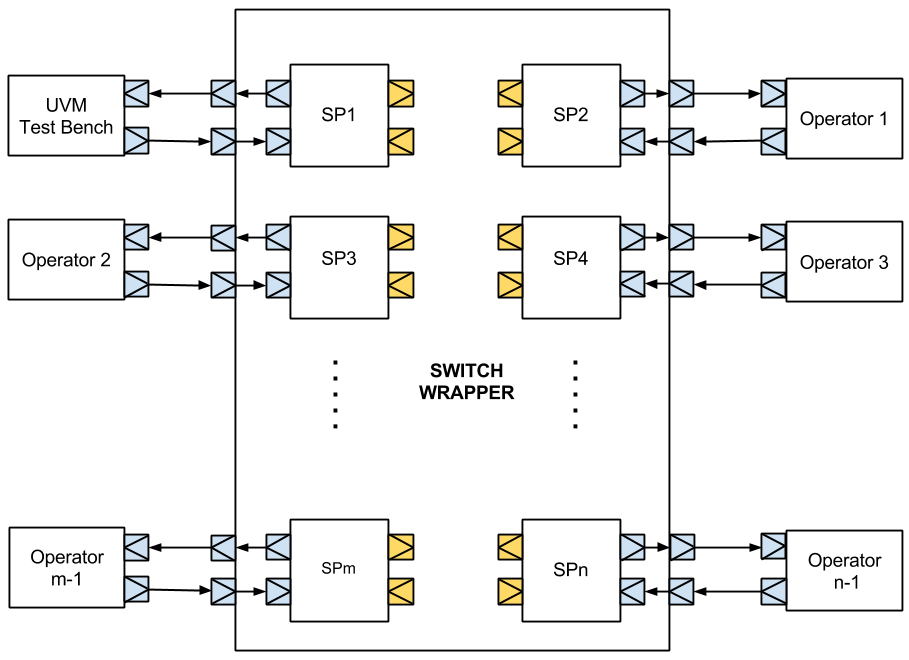
\includegraphics[scale=0.45]{testsystem}
                \caption{Complete Test System(*Multiport interconnections not shown)}
                \label{fig:testsystem}
            \end{figure}
            
            The total number of \textit{switch ports} instantiation inside \textit{switch wrapper} depends on the total \textit{Operator} units defined in the input description. The UVM environment will drive the input signals to the Freyja architecture. The Freyja interconnect consists of a 4 bytes header field and the data payload as in Fig~\ref{fig:header}. 
            In the SystemC implementation, the first byte is considered to hold the unique protocol id and the second byte to have the unique operator id, while the third byte and fourth byte are for Flow control and Context/error handling. The data bit width is suggested to be 80bits. This complete data is randomly generated with constraints from the UVM sequencer. The UVM driver will drive the input signals to the Freyja architecture.  The data is sent as a transaction payload. 
            
        
        \begin{figure}[!htb]
            \centering
            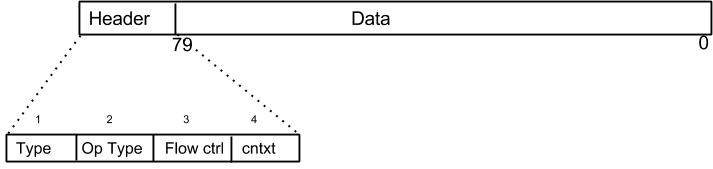
\includegraphics[scale=0.5]{header}
            \caption{FBI Interconnect}
            \label{fig:header}
        \end{figure}
        
        \subsection{Generic payload}
        
        Each generic payload transaction has a standard set of bus attributes:
        
        \begin{itemize}
        \item{\textbf{Address:} This field informs the control block of the operator unit about the source of transaction. The control block will change the address field to the destination operator address, based on the configuration data generated by Antlr.}
        \item{\textbf{Data:} The target shall copy the data to or from the data array, with respect to the semantics of other attributes. This field contains the data according to the protocol \textit{Field} section. For example, In Ethernet MAC address, payload length and data forms the Data packet.}
        \item{\textbf{Byte enables:} This is used to create burst data transfers.}
        \item{\textbf{Streaming width:} This field indicates the number of data bytes transferred on each beat in burst transfer.}
        \item{\textbf{Response status:} This field indicates the status of bus operation. The target may set the response attribute as received without errors or to one of the error type.}
        \end{itemize}

       
        \subsection{Input and Output}
        
         \begin{figure}[!htb]
             \centering
             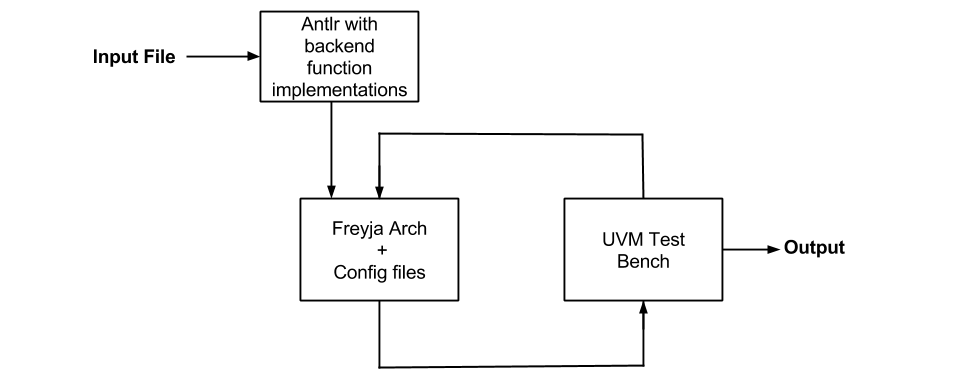
\includegraphics[scale=0.5]{inputoutput}
             \caption{Input and Output of the system}
             \label{fig:inputoutput}
            \end{figure}
    
    The input file is the description of the protocol using the developed language. The input file is parsed by the Antlr tool. The back-end functions are triggered during parsing to output the Freyja architecture and the reconfiguration files. A constrained random transaction is initiated from the UVM to the Freyja architecture and the final transaction is received back by the UVM. 
       
         \subsection{Timing annotation}
         The transaction is sent through the socket using the b\_transport method of the TLM\-2.0 blocking transport interface, which passes its transaction arguments by reference and has no return value. The b\_transport also carries the timing annotation which is not advanced, as the main interest is to model the functionality of the target and not modeling any timing detail. 
         
		\clearpage

		\section{Conclusion and future work}
        \vspace{1cm}
        \thispagestyle{plain}
        This chapter concludes the thesis by describing the learning outcomes of the reconfigurable architectures used for protocol processing and the framework design by language application. It also describes the limitations encountered during the thesis work and further section describes the future work specific to the thesis and in general to the research topic. 
        
        
        \subsection{Reconfigurable architecture} \label{rconf}
           
           Ericsson AB investigated Switch and Mesh based network topologies for efficient protocol processing. Based on performance, cost, scalability and other internal factors, switch based network topology named as Freyja is considered for further implementation and research. The reconfigurable hardware implemented using systemC consisted of a central switch with all the operators connected to it as explained in section \ref{freyja}.\\       
           
           The design of a new architecture requires manually setting up simulations, estimation of resources and synthesizing the hardware which consists of system, logic and physical synthesis. This is a time consuming process and decreases the productivity of the research. The research project called TACO (Tools for Application-specific Hardware/Software Codesign) at university of Turku explains the functions, features and capabilities required by a tool to solve these challenges \cite{taco}. One such requirement is importing architecture details in the tool from SystemC top level files. The same approach is applied in Freyja architecture by abstracting the SystemC details into the high level description.\\ 
           
           The main objective of this work is to show the complete process of mapping from high level description to the system level implementation. The features mapped consisted of different operator instantiation, interconnections, memory, error handling and routing to multiple destinations from each operator for different protocols. In general protocol processors are more complex including features like Flow control, FIFOs, arbitration mechanism, latency of each computation, dead lock avoidance etc.         
            Mapping of such finer details in the high level description will be straight forward with the approach presented in this work.
           For example, the FIFOs can be instantiated similar to the Operator instantiation by extending the language. The FIFO block can be further configured with the variable depth of the buffer and signaling the overloading because of back pressure. How these details are represented in high level description depends on the architecture implementation. The language can be extended to have the latency of each operator.\\
           
           The same framework can be used at different levels of synthesis to output the required files for the architecture. This reduces the time to reconfigure and setup the environment. For all these to be accomplish, the reconfigurable architecture should be known. The framework can be adapted based on the architecture. The approach in this work shows the concept of mapping few core features which are easy to extend for more refined details.
           
          
        \subsection{Protocol sharing} 
         
         As illustrated in section \ref{protocol}, the protocols share common functions. The features that can be shared are discussed at system level based on algorithms. The gain of sharing and reducing the hardware cost comes with the need of reconfiguration and back pressure in the system. The buffer length required to handle this and further details can be abstracted to the higher level to produce the reconfiguration content for the architecture. Automating the calculation of this resource utilization through simulation and importing the result to configure the hardware will reduce the architecture design time. \\
         
         The implemented work shows the concept of mapping one resource to different protocols. Sharing requires arbitration algorithms to decide who can access the operator at any instant of time. It can be based on priority. However mathematical tools like Matlab can be used to implement the equations and calculate the resource usage. More utilized resources like CRC computation can be replicated for avoiding the back pressure. The TACO project \cite{taco} provides a similar research conclusion for the protocol processor which exploits the resource sharing at logic levels. The tool identifies the common hardware blocks and creates multiple cores of them to meet the constraints. Similar approach can be extended with the Freyja architecture for frequently used operators.
         
      
        \subsection{Language framework}
        
        Programmers are building domain-specific languages, configuration file formats, network protocols and numerous data file formats as well as traditional programming language compilers and interpreters. The development of such systems can be made faster by using the language building tools.\\
        
        Programmers tend to avoid using language tools, resorting to adhoc methods, partly because of the raw and low level interface to these tools \cite{Bovet:2008:AAG:1410270.1410275}. Using a grammar based approach to build parsers will offer a more natural, high fidelity, robust and maintainable means of encoding a language-related problem. Most grammar development is done today with a simple text editor. The Antlr4 parser generator \cite{Parr:2007:DAR:1209320} attempts to make grammars more accessible to the programmer by generating recursive descent parsers that are very similar to what the programmer would build by hand.\\
        
        
        Antlr4 supports rapid grammar developemnt by using Antlr's built in interpreter, thus, providing immediate feedback during development \cite{Daly:2006:PES:1142473.1142568}. The parse tree associated with the matching input (as in Fig.~\ref{fig:parsetree}) helps in debugging for error in grammar definition. If the input sequence is not in the language recognized by specified start rule, Antlr4 inserts an error node into the parse tree to indicate where the problem occurred.\\ 
        
       All the above features of the Antlr4 tool helps to build the language application in a more structured way. Providing the framework in multiple languages makes the programmer comfortable to build with their preferred language. The most encountered problems are resolved with the community support and the book written by the author Terrence Parr \cite{Parr:2007:DAR:1209320}.
        
        
        \subsection{Limitations}
         
         The thesis started with the focus of developing the complete framework and to show the concept of using a language application in hardware/software co design. The reconfigurable architecture modeled in systemC abstracted more hardware details. 
         Though a language is developed to include all future requirements, the implementations in the backend have to be extended for the new features of the hardware. Even though three protocols and their functions are discussed, integration of only Ethernet and part of Xio-s protocol is considered. As stated in section \ref{rconf}, the high level description is targeted with respect to the current Freyja architecture. The Antlr4 tool supports Java language and other languages are yet to be released.
         
         \subsection{Future work}
        
          The Freyja architecture is still under implementation and in the future, the complete details of the architecture can be abstracted into high level description by extending the language. Features like multiple core instantiations and transactions from different sources to same destination (required for Xio-s protocol) are possible to represent but still require the backend implementations to modify according to the interconnection defined in future. Once the reconfigurable file format required by RTL hardware implementations is defined, the same framework can output such files to speedup the design process. As explained in section \ref{reconf}, the granularity of Freyja architecture is at algorithmic level. Exploiting the reconfigurability for the Freyja architecture can be considered further with respect to common hardware blocks at logic levels and then the language can be extended similar to the TACO protocol processor \cite{taco}. The header, as depicted in Fig.~\ref{fig:header}, can be described in the high level description which provides control in manipulating the length of each field.\\
          
          The integration of Xio-s and CPRI protocols into the framework is straight forward. The process block that is the core functions of each operator needs to be modified to integrate these protocols into the system. Antlr4 is made to output the framework in Java language and the tool (in future!) will support other languages like C and C++. Based on the project requirements the language can be selected. Java has good commands for file IO operations and object handling. The major back-end implementation deals with storing the parsed data in the form of hash-map and linked-list. These facts can be considered when building similar concepts for other reconfigurable architectures. \\ 
        
         
          In general, the framework can be extended for all levels of synthesis while designing the hardware. The development environment will be heterogeneous at different levels and a common framework for producing the top level configurable files will reduce the errors. Once the architecture is specified, the tool can be made to generate the SystemC model for simulation, a Matlab model for estimation of resources and a VHDL model for synthesis of the architecture. The resource estimation can also be integrated within the tool by developing an interpreter using the parsed input. 
         
             
        
		\clearpage

	\begin{filecontents*}{references.bib}


		@INPROCEEDINGS{5335678, 
			author={Szczesny, D. and Showk, A. and Hessel, S. and Bilgic, A. and Hildebrand, U. and Frascolla, V.}, 
			booktitle={System-on-Chip, 2009. SOC 2009. International Symposium on}, 
			title={Performance analysis of LTE protocol processing on an ARM based mobile platform}, 
			year={2009}, 
			month={Oct}, 
			pages={056-063}, 
			keywords={hardware-software codesign;mobile communication;mobile handsets;virtual prototyping;ARM based mobile platform;LTE protocol processing;long term evolution layer;robust header compression;Acceleration;Computational modeling;Hardware;Long Term Evolution;Mobile computing;Mobile handsets;Performance analysis;Physical layer;Protocols;Virtual prototyping}, 
			doi={10.1109/SOCC.2009.5335678},}

			@INPROCEEDINGS{558379, 
				author={Abnous, A. and Rabaey, J.}, 
				booktitle={VLSI Signal Processing, IX, 1996., [Workshop on]}, 
				title={Ultra-low-power domain-specific multimedia processors}, 
				year={1996}, 
				month={Oct}, 
				pages={461-470}, 
				keywords={computer architecture;computer networks;digital signal processing chips;integrated circuit design;land mobile radio;mobile radio;multimedia communication;portable computers;radio equipment;communication capabilities;hybrid architecture template;multimedia services;portable communication devices;portable computing;programmable devices;signal processing applications;ultra-low-power domain-specific multimedia processors;Computer aided instruction;Computer architecture;Decoding;Digital signal processing;Energy efficiency;Kernel;Multimedia computing;Portable computers;Power engineering computing;Signal processing algorithms}, 
				doi={10.1109/VLSISP.1996.558379},}

				@INPROCEEDINGS{1106752, 
					author={Keutzer, K. and Malik, S. and Newton, A.R.}, 
					booktitle={Computer Design: VLSI in Computers and Processors, 2002. Proceedings. 2002 IEEE International Conference on}, 
					title={From ASIC to ASIP: the next design discontinuity}, 
					year={2002}, 
					month={}, 
					pages={84-90}, 
					keywords={application specific integrated circuits;logic design;programmable circuits;ASIC;ASIP;Application Specific Instruction Set Processors;Application Specific Integrated Circuits;application implementation philosophy;programmable platforms;Application software;Application specific integrated circuits;Application specific processors;Computational geometry;Costs;Design methodology;Hardware;Manufacturing;Productivity;Time to market}, 
					doi={10.1109/ICCD.2002.1106752}, 
					ISSN={1063-6404},}

					@INPROCEEDINGS{6868627, 
						author={Badawi, M. and Hemani, A. and Zhonghai Lu}, 
						booktitle={Application-specific Systems, Architectures and Processors (ASAP), 2014 IEEE 25th International Conference on}, 
						title={Customizable coarse-grained energy-efficient reconfigurable packet processing architecture}, 
						year={2014}, 
						month={June}, 
						pages={30-35}, 
						keywords={application specific integrated circuits;multiprocessing systems;reconfigurable architectures;agile reconfigurability;custom ASIC implementation;customizable coarse grained energy efficient reconfigurable packet processing architecture;hardwired ASIC implementation;programmable protocol processor;real-life Voice-Over IP traffic;reconfigurable multicore packet processing architecture;retaining flexibility;time critical adaptability;Application specific integrated circuits;Delays;IP networks;Program processors;Protocols;Registers;Time factors}, 
						doi={10.1109/ASAP.2014.6868627},}

						@ARTICLE{1114865, 
							author={Estrin, G.}, 
							journal={Annals of the History of Computing, IEEE}, 
							title={Reconfigurable computer origins: the UCLA fixed-plus-variable (F+V) structure computer}, 
							year={2002}, 
							month={Oct}, 
							volume={24}, 
							number={4}, 
							pages={3-9}, 
							keywords={reconfigurable architectures;UCLA fixed-plus-variable structure computer;University of California at Los Angeles;models;reconfigurable computer architectures;reconfigurable systems analysis;reconfigurable systems design;tools;Circuits;Computer architecture;Contracts;Hardware;High performance computing;Laboratories;Mathematics;Microprocessors;System analysis and design;Telephony}, 
							doi={10.1109/MAHC.2002.1114865}, 
							ISSN={1058-6180},}

							@misc{page1985re,
								title={Re-programmable PLA},
								author={Page, D.W. and Peterson, L.V.R.},
								url={http://www.google.com/patents/US4508977},
								year={1985},
								month=apr # "~2",
								publisher={Google Patents},
								note={US Patent 4,508,977}
							}

                        @article{JACST518,
	                    author = {Abida Waza and Roohie Naaz Mir and Hakim Najeeb-ud-din},
	                    title = {Reconfigurable Architectures},
	                    journal = {Journal of Advanced Computer Science \& Technology},
                    	volume = {1},
	                    number = {4},
                    	year = {2012},
	                    keywords = {},
	                    abstract = {In the area of computer architecture, designers are faced with the trade-of between flexibility and performance. The architectural choices span a wide spectrum, with general-purpose processors and application specific integrated circuits (ASICs) at opposite ends. General-purpose processors are not optimized to specific applications; they are flexible due to their versatile instruction sets that allow the implementation of every computable task. ASICs are dedicated hardware devices that can achieve higher performance, require less silicon area, and are less power-consuming than instruction-level programmable processors. However, they lack in flexibility. Reconfigurable computer architectures promise to overcome this traditional trade-off and achieve both, the high performance of ASICs and the flexibility of general-purpose processors.},
	                    issn = {2227-4332},
	                    url = {http://www.sciencepubco.com/index.php/JACST/article/view/518},
	                    pages = {337--346}}

                    	@INPROCEEDINGS{5351593, 
	                	author={Shami, M.A. and Hemani, A.}, 
	                	booktitle={ASIC, 2009. ASICON '09. IEEE 8th International Conference on}, 
		                title={Partially reconfigurable interconnection network for dynamically reprogrammable resource array}, 
		                year={2009}, 
		                month={Oct}, 
	                	pages={122-125}, 
	                	keywords={multiprocessor interconnection networks;reconfigurable architectures;binary encoding;dynamically reprogrammable resource array;innovative regular nonblocking interconnection network;low latency interconnection network;partially reconfigurable interconnection network;point-to-multipoint interconnection network;point-to-point interconnection network;sliding window connectivity;Delay;Energy efficiency;Fabrics;Multiplexing;Multiprocessor interconnection networks;Nearest neighbor searches;Parallel processing;Reconfigurable architectures;Reconfigurable logic;Signal processing algorithms;CGRA;Dynamically Reconfigurable;Interconnects;Partially Reconfigurable}, 
		                doi={10.1109/ASICON.2009.5351593},}
                    
                    
                         @comment{ Anne H�kansson, Portal of Research Methods and Methodologies for 
                             Research Projects and Degree Projects. WORLDCOMP'13 - The 2013 
                             World Congress in Computer Science, Computer Engineering, and 
                             Applied Computing, 22-25 July, 2013 Las Vegas, Nevada; USA }
                            @book{2013portal,
                                author = "Anne H�kansson",
                                title = "Portal of Research Methods and Methodologies for Research Projects and Degree Projects",
                                publisher = "WORLDCOMP'13 - The 2013 World Congress in Computer Science, Computer Engineering, and Applied Computing",
                                pages = "22--25",
                                year = 2013
                            }
                            
                           @ARTICLE{1617814, 
                               journal={IEEE Std 1666-2005}, 
                               title={IEEE Standard System C Language Reference Manual}, 
                               year={2006}, 
                               month={}, 
                               pages={0\_1-423}, 
                               doi={10.1109/IEEESTD.2006.99475},}
                            
                           @ARTICLE{4066263, 
                               author={Peterson, W.W. and Brown, D.T.}, 
                               journal={Proceedings of the IRE}, 
                               title={Cyclic Codes for Error Detection}, 
                               year={1961}, 
                               month={Jan}, 
                               volume={49}, 
                               number={1}, 
                               pages={228-235}, 
                               keywords={Binary codes;Data communication;Decoding;Encoding;Error correction codes;Feedback;Fires;Information theory;Mathematics;Polynomials}, 
                               doi={10.1109/JRPROC.1961.287814}, 
                               ISSN={0096-8390},}
                            
                            
                           @MISC{antlr4,
                               author = {Terence Parr, Sam Harwell and Kathleen Fisher},
                               title = {Adaptive LL(*) Parsing: The Power of Dynamic Analysis},
                               month = March,
                               year = {2014},
                               howpublished = "\url{http://www.antlr.org/papers/allstar-techreport.pdf}",
                               note = "[Online; accessed 1-March-2015]",
                               url = {http://www.antlr.org/papers/allstar-techreport.pdf}}
                            
                            
                          @INPROCEEDINGS{4291932, 
                              author={Genest, G. and Chamberlain, R. and Bruce, R.}, 
                              booktitle={Adaptive Hardware and Systems, 2007. AHS 2007. Second NASA/ESA Conference on}, 
                              title={Programming an FPGA-based Super Computer Using a C-to-VHDL Compiler: DIME-C}, 
                              year={2007}, 
                              month={Aug}, 
                              pages={280-286}, 
                              keywords={field programmable gate arrays;hardware description languages;logic CAD;parallel machines;program compilers;programming;64-node FPGA-based supercomputer programming;C-to-VHDL compiler;Nallatech DIME-C compiler;design methodology;ANSI standards;Algorithm design and analysis;Circuits;Electronic design automation and methodology;Field programmable gate arrays;Hardware design languages;High level languages;Logic;Pipelines;Program processors}, 
                              doi={10.1109/AHS.2007.89},}
                            
                            
                            
                          @ARTICLE{998629, 
                              author={Bergamaschi, R.}, 
                              journal={Computer-Aided Design of Integrated Circuits and Systems, IEEE Transactions on}, 
                              title={Bridging the domains of high-level and logic synthesis}, 
                              year={2002}, 
                              month={May}, 
                              volume={21}, 
                              number={5}, 
                              pages={582-596}, 
                              keywords={data flow graphs;high level synthesis;logic CAD;minimisation of switching nets;processor scheduling;RTL/gate-level network;algorithmic decision;allocation;control/data flow graphs;hardware cost estimation;hardware implementation;high-level synthesis;interleaving;internal model;logic synthesis;logic transformations;register-transfer-level model;scheduling;Costs;Flow graphs;Hardware;High level synthesis;Logic design;Logic gates;Network synthesis;Processor scheduling;Resource management;Scheduling algorithm}, 
                              doi={10.1109/43.998629}, 
                              ISSN={0278-0070},}
                            
                            
                            @INPROCEEDINGS{5469564, 
                                author={Mena, J.G. and Deken, R. and Coker, J.E. and Johnstone, M.S. and Ramirez, S.R. and Frey, P.}, 
                                booktitle={VLSI Test Symposium (VTS), 2010 28th}, 
                                title={High level synthesis of a Front End filter and DSP engine for analog to digital conversion x2013; a case study}, 
                                year={2010}, 
                                month={April}, 
                                pages={252-252}, 
                                keywords={analogue-digital conversion;digital signal processing chips;electronic engineering computing;high level synthesis;object-oriented programming;SystemC;analog to digital conversion;front end DSP engine;front end filter;high level synthesis;object oriented programming;sine cubed decimator;Analog-digital conversion;Digital filters;Digital signal processing;Engines;High level synthesis;Microarchitecture;Object oriented modeling;Productivity;Silicon compiler;Timing}, 
                                doi={10.1109/VTS.2010.5469564}, 
                                ISSN={1093-0167},}
                            
                            @INPROCEEDINGS{5681536, 
                                author={Kaneta, Y. and Yoshizawa, S. and Minato, S. and Arimura, H. and Miyanaga, Y.}, 
                                booktitle={Field-Programmable Technology (FPT), 2010 International Conference on}, 
                                title={Dynamic reconfigurable bit-parallel architecture for large-scale regular expression matching}, 
                                year={2010}, 
                                month={Dec}, 
                                pages={21-28}, 
                                keywords={deterministic automata;field programmable gate arrays;finite automata;parallel architectures;random-access storage;reconfigurable architectures;string matching;DFA-based dynamic reconfigurable architectures;FPGA-based architecture;bit-masks;bit-parallel NFA-simulation;bit-parallel pattern matching approach;block RAM;dynamic BP-NFA;dynamic reconfigurable bit-parallel NFA architecture;dynamic reconfigurable bit-parallel architecture;large-scale regular expression matching;nondeterministic finite automata;string matching;Decoding;Field programmable gate arrays;Hardware;Indexes;Pattern matching;Random access memory;Registers}, 
                                doi={10.1109/FPT.2010.5681536},}
                            
                            @INPROCEEDINGS{1395538, 
                                author={Panainte, E.M. and Bertels, K. and Vassiliadis, S.}, 
                                booktitle={Design, Automation and Test in Europe, 2005. Proceedings}, 
                                title={Instruction scheduling for dynamic hardware configurations [M-JPEG encoder case study]}, 
                                year={2005}, 
                                month={March}, 
                                pages={100-105 Vol. 1}, 
                                keywords={directed graphs;discrete cosine transforms;field programmable gate arrays;processor scheduling;quantisation (signal);reconfigurable architectures;variable length codes;video coding;DCT;FCCM;FPGA area placement conflicts;FPGA reconfiguration latency;M-JPEG encoder speedup;compiler analyses techniques;control flow graph;directed graph;dynamic hardware configuration;executed hardware reconfiguration instructions minimization;feedback-directed techniques;field-programmable custom computing machines;instruction scheduling algorithm;operation hardware execution;operation software execution;quantization;variable length coding;Algorithm design and analysis;Application software;Delay;Dynamic scheduling;Field programmable gate arrays;Hardware;Scheduling algorithm;Software algorithms;Switches;Testing}, 
                                doi={10.1109/DATE.2005.184}, 
                                ISSN={1530-1591},}
                           
                                               
                        
                                                      
                            
                          @MISC{ericsson,
                              author = {},
                              title = {Ericsson AB},
                              month = July,
                              year = {2015},
                              howpublished = "\url{http://www.ericsson.com/}",
                              note = "[Online; accessed 1-March-2015]",
                              url = {http://www.ericsson.com/}}
                          
                          
                        @MISC{gaut,
                            author = {},
                            title = {},
                            month = sept,
                            year = {2015},
                            howpublished = "\url{http://hls-labsticc.univ-ubs.fr/}",
                            note = "[Online; accessed 20-Sept-2015]",
                            url = {http://hls-labsticc.univ-ubs.fr/}}       
                            
                            
                            
                        @MISC{xilinx,
                            author = {},
                            title = {Xilinx, All programmable},
                            month = Aug,
                            year = {2015},
                            howpublished = "\url{http://www.xilinx.com/fpga/}",
                            note = "[Online; accessed 1-Sept-2015]",
                            url = {http://www.xilinx.com/fpga/}}  
                            
                            
                            
                        @MISC{iethernet,
                            author = {},
                            title = {IEEE Standard for Ethernet},
                            month = July,
                            year = {2012},
                            howpublished = "\url{https://standards.ieee.org/about/get/802/802.3.html}",
                            note = "[Online; accessed 1-Feb-2015]",
                            url = {https://standards.ieee.org/about/get/802/802.3.html}}    
                          
                        @MISC{cpri,
                              author = {},
                              title = {CPRI specification overview},
                              month = July,
                              year = {2014},
                              howpublished = "\url{http://www.cpri.info/spec.html}",
                              note = "[Online; accessed 1-Feb-2015]",
                              url = {http://www.cpri.info/spec.html}}  
                          
                        @incollection{book,
                            year={2011},
                            isbn={978-1-4419-8585-9},
                            booktitle={The Simple Art of SoC Design},
                            doi={10.1007/978-1-4419-8586-6_12},
                            title={The Future of Design},
                            url={http://dx.doi.org/10.1007/978-1-4419-8586-6_12},
                            publisher={Springer New York},
                            author={Keating, Michael},
                            pages={171-180},
                            language={English}
                          }  
                          
                         
                          @MISC{tlm,
                              author = {},
                              title = {TLM 2.0 Transaction Level Modeling Library and whitepaper},
                              month = July,
                              year = {2009},
                              howpublished = "\url{http://accellera.org/downloads/standards/systemc}",
                              note = "[Online; accessed 1-Feb-2015]",
                              url = {http://accellera.org/downloads/standards/systemc}}  
                         
                           @MISC{uvm,
                               author = {},
                               title = {Standard Universal Verification Methodology Class Reference},
                               month = July,
                               year = {2014},
                               howpublished = "\url{ http://accellera.org/downloads/standards/uvm}",
                               note = "[Online; accessed 1-Feb-2015]",
                               url = { http://accellera.org/downloads/standards/uvm}}   
                            
                            @MISC{sematech,
                                author = {Semiconductor Industry Association},
                                title = {The International Technology Roadmap for Semiconductors SEMATECH: Austin, 2009},
                                month = July,
                                year = {2009}}
                               
                               
                               
                            @InProceedings{taco,
                                author = {Seppo Virtanen and Tomas Lundstr�om and Johan Lilius},
                                title = {A Design Tool for the TACO Protocol
                                    Processor Development Framework},
                                booktitle = {n Proceedings of the 18 IEEE NorChip conference, 6-7 November 2000, Turku, Finland },
                                month =,
                                year = ,
                                publisher = {},
                                editor = {},
                                pages = {},}
                            
                         @article{Bovet:2008:AAG:1410270.1410275,
                             author = {Bovet, Jean and Parr, Terence},
                             title = {ANTLRWorks: An ANTLR Grammar Development Environment},
                             journal = {Softw. Pract. Exper.},
                             issue_date = {October 2008},
                             volume = {38},
                             number = {12},
                             month = oct,
                             year = {2008},
                             issn = {0038-0644},
                             pages = {1305--1332},
                             numpages = {28},
                             url = {http://dx.doi.org/10.1002/spe.v38:12},
                             doi = {10.1002/spe.v38:12},
                             acmid = {1410275},
                             publisher = {John Wiley \& Sons, Inc.},
                             address = {New York, NY, USA},
                             keywords = {GUI, debugger, grammar development, parser, rapid prototyping},
                            } 
                         
                         @book{Parr:2007:DAR:1209320,
                             author = {Parr, Terence},
                             title = {The Definitive ANTLR Reference: Building Domain-Specific Languages},
                             year = {2007},
                             isbn = {0978739256},
                             publisher = {Pragmatic Bookshelf},
                         }   
                         
                         @inproceedings{Daly:2006:PES:1142473.1142568,
                             author = {Daly, Mark and Mandelbaum, Yitzhak and Walker, David and Fern\'{a}ndez, Mary and Fisher, Kathleen and Gruber, Robert and Zheng, Xuan},
                             title = {PADS: An End-to-end System for Processing Ad Hoc Data},
                             booktitle = {Proceedings of the 2006 ACM SIGMOD International Conference on Management of Data},
                             series = {SIGMOD '06},
                             year = {2006},
                             isbn = {1-59593-434-0},
                             location = {Chicago, IL, USA},
                             pages = {727--729},
                             numpages = {3},
                             url = {http://doi.acm.org/10.1145/1142473.1142568},
                             doi = {10.1145/1142473.1142568},
                             acmid = {1142568},
                             publisher = {ACM},
                             address = {New York, NY, USA},
                            } 
                         
                          @book{hls,
                              author = {Philippe Coussy, Adam Morawiec},
                              title = {High-Level Synthesis: From Algorithm to Digital Circuit},
                              year = {2008},
                              isbn = {978-1-4020-8588-8},
                              publisher = {Springer Netherlands},
                            } 
                            
                            @book{groundup,
                                author = {David C. Black, Jack Donovan},
                                title = {SystemC: From the Ground Up},
                                year = {2004},
                                isbn = {978-0-387-30864-7},
                                publisher = {Springer US},
                               }  
                           
                           
                           
                         
                         @ARTICLE{5209958, 
                             author={Coussy, P. and Gajski, D.D. and Meredith, M. and Takach, A.}, 
                             journal={Design Test of Computers, IEEE}, 
                             title={An Introduction to High-Level Synthesis}, 
                             year={2009}, 
                             month={July}, 
                             volume={26}, 
                             number={4}, 
                             pages={8-17}, 
                             keywords={high level synthesis;HLS techniques;abstraction level design;high-level synthesis;optimized RTL hardware;Application software;Assembly;Circuit simulation;Circuit synthesis;Computer architecture;Design methodology;Design optimization;Hardware design languages;High level synthesis;Space exploration;RTL abstraction;architectures;custom processors;design and test;hardware synthesis and verification;high-level synthesis}, 
                             doi={10.1109/MDT.2009.69}, 
                             ISSN={0740-7475},}
                            
                         @INPROCEEDINGS{5382069, 
                             author={Mayer-Lindenberg, F.}, 
                             booktitle={Reconfigurable Computing and FPGAs, 2009. ReConFig '09. International Conference on}, 
                             title={High-Level FPGA Programming through Mapping Process Networks to FPGA Resources}, 
                             year={2009}, 
                             month={Dec}, 
                             pages={302-307}, 
                             keywords={codes;field programmable gate arrays;microprocessor chips;program compilers;FPGA based scalable processor networks;FPGA configuration bitstream;close-to-interactive speeds;coarse-grained processor network;floating point processing;high-level FPGA programming;high-level programming interface;mixed multicomponent FPGA;p-Nets language;process network mapping;program code;Arithmetic;Computer networks;Costs;Delay;Field programmable gate arrays;Hardware design languages;Integrated circuit interconnections;Libraries;Routing;SDRAM}, 
                             doi={10.1109/ReConFig.2009.73},}
                            
                            
                       
                       @INPROCEEDINGS{1303110, 
                           author={Schaumont, P. and Sakiyama, K. and Hodjat, A. and Verbauwhede, I.}, 
                           booktitle={Parallel and Distributed Processing Symposium, 2004. Proceedings. 18th International}, 
                           title={Embedded software integration for coarse-grain reconfigurable systems}, 
                           year={2004}, 
                           month={April}, 
                           pages={137-}, 
                           keywords={coprocessors;embedded systems;integrated software;reconfigurable architectures;system-on-chip;coarse-grain reconfigurable system;embedded software integration;energy-efficiency improvement;network-on-chip system;network-processing acceleration unit;processor network;programming complexity;run-time reconfiguration mechanism;tightly-coupled coprocessor;Acceleration;Application software;Coprocessors;Costs;Cryptography;Embedded software;Energy efficiency;Hardware;Runtime;Software systems}, 
                           doi={10.1109/IPDPS.2004.1303110},}
                        
                        @ARTICLE{839320, 
                            author={DeHon, A.}, 
                            journal={Computer}, 
                            title={The density advantage of configurable computing}, 
                            year={2000}, 
                            volume={33}, 
                            number={4}, 
                            pages={41-49}, 
                            keywords={field programmable gate arrays;reconfigurable architectures;DNA sequence matching;FPGAs;RSA decryption;absolute performance;configurable computing;configurable machines;cryptographic attacks;emulation;programmable computing;signal processing;Acceleration;Array signal processing;Computer applications;Cryptography;DNA computing;Digital signal processing;Emulation;Field programmable gate arrays;Microprocessors;Sequences}, 
                            doi={10.1109/2.839320}, 
                            ISSN={0018-9162}, 
                            month={Apr},}
                        
                                               
                        @ARTICLE{1654264, 
                            author={Gajski, D.D. and Kuhn, R.H.}, 
                            journal={Computer}, 
                            title={Guest Editors' Introduction: New VLSI Tools}, 
                            year={1983}, 
                            volume={16}, 
                            number={12}, 
                            pages={11-14}, 
                            keywords={Algorithm design and analysis;Computer graphics;Design automation;Design optimization;Expert systems;Integrated circuit synthesis;Programmable logic arrays;Special issues and sections;Very large scale integration}, 
                            doi={10.1109/MC.1983.1654264}, 
                            ISSN={0018-9162}, 
                            month={Dec},}
                        
                        @inproceedings{ARM:07,
                            author = {Chulho Shin and Peter Grun and Nizar Romdhane and Christopher Lennard and Gabor Madl and Sudeep Pasricha and Nikil Dutt and Mark Noll},
                            title = {{Enabling heterogeneous cycle-based and event-driven simulation in a design flow integrated using the SPIRIT consortium specifications}},
                            journal = {{Design Automation for Embedded Systems}},
                            volume = {11},
                            number = {2--3},
                            year = {2007},
                            month = {September}
                        }
                        
                        
                        @incollection{cgra,
                            year={2007},
                            isbn={978-1-4020-6504-0},
                            booktitle={Fine- and Coarse-Grain Reconfigurable Computing},
                            editor={Vassiliadis, Stamatis and Soudris, Dimitrios},
                            doi={10.1007/978-1-4020-6505-7\_2},
                            title={A Survey of Coarse-Grain Reconfigurable Architectures and Cad Tools},
                            url={http://dx.doi.org/10.1007/978-1-4020-6505-7\_2},
                            publisher={Springer Netherlands},
                            keywords={Coarse-grain reconfigurable systems/architectures; design issues of coarse-grain reconfigurable systems; mapping/compilation methods; reconfiguration mechanisms},
                            author={Theodoridis, G. and Soudris, D. and Vassiliadis, S.},
                            pages={89-149},
                            language={English}
                        }
                        
                        @ARTICLE{4469916, 
                            author={Dongwan Shin and Gerstlauer, A. and Domer, R. and Gajski, D.D.}, 
                            journal={Very Large Scale Integration (VLSI) Systems, IEEE Transactions on}, 
                            title={An Interactive Design Environment for C-Based High-Level Synthesis of RTL Processors}, 
                            year={2008}, 
                            volume={16}, 
                            number={4}, 
                            pages={466-475}, 
                            keywords={C language;embedded systems;high level synthesis;pipeline processing;system-on-chip;C language;RTL processor;binding;chaining;clock definition;component allocation;embedded system;high-level synthesis;interactive RTL design environment;multicycling;pipelining;processor architecture;register transfer level;scheduling;system-on-chip;Embedded systems;high level synthesis;interactive design environment;register transfer level (RTL) processor;system-on-chip (SoC)}, 
                            doi={10.1109/TVLSI.2007.915390}, 
                            ISSN={1063-8210}, 
                            month={April},}
                         
                         
                         
                         @INPROCEEDINGS{1188678, 
                             author={Bingfeng Mei and Vernalde, S. and Verkest, D. and De Man, H. and Lauwereins, R.}, 
                             booktitle={Field-Programmable Technology, 2002. (FPT). Proceedings. 2002 IEEE International Conference on}, 
                             title={DRESC: a retargetable compiler for coarse-grained reconfigurable architectures}, 
                             year={2002}, 
                             pages={166-173}, 
                             keywords={circuit layout CAD;embedded systems;high level synthesis;parallel architectures;processor scheduling;reconfigurable architectures;DRESC;architecture abstraction;coarse-grained reconfigurable architectures;dataflow;internal graph representation;modulo scheduling algorithm;program analysis;retargetable compiler;scheduling;Computer architecture;Concrete;Field programmable gate arrays;Kernel;Parallel processing;Reconfigurable architectures;Scheduling algorithm;Testing;Topology;VLIW}, 
                             doi={10.1109/FPT.2002.1188678}, 
                             month={Dec},}
                            
                            @inproceedings{1530618,
                                author = {Alle, Mythri and Varadarajan, Keshavan and Fell, Alexander and Nandy, S. K. and Narayan, Ranjani},
                                title = {Compiling Techniques for Coarse Grained Runtime Reconfigurable Architectures},
                                booktitle = {Proceedings of the 5th International Workshop on Reconfigurable Computing: Architectures, Tools and Applications},
                                series = {ARC '09},
                                year = {2009},
                                isbn = {978-3-642-00640-1},
                                location = {Karlsruhe, Germany},
                                pages = {204--215},
                                numpages = {12},
                                url = {http://dx.doi.org/10.1007/978-3-642-00641-8_21},
                                doi = {10.1007/978-3-642-00641-8_21},
                                acmid = {1530618},
                                publisher = {Springer-Verlag},
                                address = {Berlin, Heidelberg},
                            } 
                            
                            @INPROCEEDINGS{5669439, 
                                author={Malik, O. and Hemani, A. and Shami, M.A.}, 
                                booktitle={NORCHIP, 2010}, 
                                title={High Level Synthesis Framework for a Coarse Grain Reconfigurable Architecture}, 
                                year={2010}, 
                                pages={1-6}, 
                                keywords={digital signal processing chips;high level synthesis;reconfigurable architectures;DSP algorithms;SIMD;coarse grain reconfigurable architecture;high level synthesis framework;Computer architecture;Digital signal processing;Finite impulse response filter;Resource management;Synchronization;CGRA;High Level Language;High level synthesis;Symbolic Assembler}, 
                                doi={10.1109/NORCHIP.2010.5669439}, 
                                month={Nov},}
                            
                            @INPROCEEDINGS{707889, 
                                author={Cronquist, D.C. and Franklin, P. and Berg, S.G. and Ebeling, C.}, 
                                booktitle={FPGAs for Custom Computing Machines, 1998. Proceedings. IEEE Symposium on}, 
                                title={Specifying and compiling applications for RaPiD}, 
                                year={1998}, 
                                pages={116-125}, 
                                keywords={decoding;field programmable gate arrays;formal specification;reconfigurable architectures;RaPiD;computation-intensive applications;control program;decoding structure;deeply pipelined implementations;dynamic control signals;flexible architectures;pipelined computation structures;reconfigurable pipelined datapath architecture;special-purpose hardware machines;statically configured datapath;Application software;Circuits;Computer applications;Computer architecture;Computer science;Decoding;Hardware;High level languages;Pipelines;Program processors}, 
                                doi={10.1109/FPGA.1998.707889}, 
                                month={Apr},}
                            
                            
                            @ARTICLE{839324, 
                                author={Goldstein, S.C. and Schmit, H. and Budiu, M. and Cadambi, S. and Moe, M. and Taylor, R.R.}, 
                                journal={Computer}, 
                                title={PipeRench: a reconfigurable architecture and compiler}, 
                                year={2000}, 
                                volume={33}, 
                                number={4}, 
                                pages={70-77}, 
                                keywords={performance evaluation;program compilers;reconfigurable architectures;FPGA architectures;PipeRench;compilation time;compiler;configuration time;custom hardware;digital signal processor;efficiency;embedded computer systems;flexibility;forward compatibility;general-purpose processors;hard constraints;logic granularity;microcontroller;performance speedup;reconfigurable architecture;reconfigurable computing;Application software;Computer architecture;Digital signal processors;Embedded computing;Field programmable gate arrays;Hardware;Microcontrollers;Reconfigurable architectures;Reconfigurable logic;Time factors}, 
                                doi={10.1109/2.839324}, 
                                ISSN={0018-9162}, 
                                month={Apr},}
                            
                            @INPROCEEDINGS{Abnous98evaluationof,
                                author = {Arthur Abnous and Katsunori Senoy and Marlene Wan and Jan Rabaey},
                                title = {Evaluation of a low-power reconfigurable DSP architecture},
                                booktitle = {proceedings 5 th Reconfigurable Architectures workshop (RAW98), March 30},
                                year = {1998},
                                pages = {55--60},
                                publisher = {Springer}
                            }
                            
                             @INPROCEEDINGS{progril,
                                 author = {R.H.J Bloks},
                                 title = {A Grammar Based Approach towards the automatic implementation of Data Communication protocols in Hardware},
                                 booktitle = {Ph. D thesis, Eindhoven University of Technology, Sept 1993},
                                 year = {1993},
                                 pages = {},
                                 publisher = {}
                                }
                            
                            @INPROCEEDINGS{1213333, 
                                author={Heysters, P.M. and Smit, G.J.M.}, 
                                booktitle={Parallel and Distributed Processing Symposium, 2003. Proceedings. International}, 
                                title={Mapping of DSP algorithms on the MONTIUM architecture}, 
                                year={2003}, 
                                pages={6 pp.-}, 
                                keywords={digital signal processing chips;parallel algorithms;parallel architectures;reconfigurable architectures;system-on-chip;DSP algorithm mapping;MONTIUM architecture;battery operated mobile devices;course-grained reconfigurable architecture;digital signal processing algorithms;flexible high-performance architectures;programmable systems;Computer architecture;Digital signal processing;Energy efficiency;Hardware;Kernel;Reconfigurable architectures;Registers;Signal processing algorithms;Tiles;VLIW}, 
                                doi={10.1109/IPDPS.2003.1213333}, 
                                ISSN={1530-2075}, 
                                month={April},}
                            
                            @ARTICLE{831438, 
                                author={Oberg, J. and Kumar, A. and Hemani, A.}, 
                                journal={Very Large Scale Integration (VLSI) Systems, IEEE Transactions on}, 
                                title={Grammar-based hardware synthesis from port-size independent specifications}, 
                                year={2000}, 
                                volume={8}, 
                                number={2}, 
                                pages={184-194}, 
                                keywords={grammars;high level synthesis;protocols;ATM;Program;automaton;communication protocol;grammar-based language;hardware synthesis;port-size independent specification;system design;Application software;Automata;Books;Computer languages;Hardware design languages;High level synthesis;Java;Protocols;Space exploration;Testing}, 
                                doi={10.1109/92.831438}, 
                                ISSN={1063-8210}, 
                                month={April},}
                            
                            @INPROCEEDINGS{565871, 
                                author={Oberg, J. and Kumar, A. and Hemani, A.}, 
                                booktitle={System Synthesis, 1996. Proceedings., 9th International Symposium on}, 
                                title={Grammar-based hardware synthesis of data communication protocols}, 
                                year={1996}, 
                                pages={14-19}, 
                                keywords={data communication;high level synthesis;logic design;protocols;specification languages;PRO-GRAM;VHDL-code;compiler;data communication protocols;design space exploration;grammar-based hardware synthesis;hardware specification;implementation independent design specification;logic synthesis;protocol specification language;synthesis methodology;tokens;Circuit synthesis;Control system synthesis;Data communication;Hardware;High level synthesis;Laboratories;Protocols;Space exploration;Space technology;Telephony}, 
                                doi={10.1109/ISSS.1996.565871}, 
                                ISSN={1080-1820}, 
                                month={Nov},}
                            
                            @INPROCEEDINGS{1012696, 
                                author={Siegmund, R. and Muller, D.}, 
                                booktitle={Design Automation Conference, 2002. Proceedings. 39th}, 
                                title={A novel synthesis technique for communication controller hardware from declarative data communication protocol specifications}, 
                                year={2002}, 
                                pages={602-607}, 
                                keywords={asynchronous transfer mode;controller area networks;flow graphs;formal specification;high level synthesis;protocols;ATM;C++ code;CAN;COSYNE tool;IEC14443 Wireless SmartCard;RTL models;USB;bit-serial protocols;communication controller hardware synthesis;conformity;consumer controllers;data communication protocol specifications;formal specification;interacting transaction producer;interconnect;interface-based design;protocol flow graph;single protocol specification;Algorithm design and analysis;Circuit synthesis;Communication system control;Control system synthesis;Control systems;Data communication;Hardware;Permission;Protocols;Universal Serial Bus}, 
                                doi={10.1109/DAC.2002.1012696}, 
                                ISSN={0738-100X}, 
                                month={},}
                            
                            @ARTICLE{285744, 
                                author={Seawright, A. and Brewer, F.}, 
                                journal={Very Large Scale Integration (VLSI) Systems, IEEE Transactions on}, 
                                title={Clairvoyant: a synthesis system for production-based specification}, 
                                year={1994}, 
                                volume={2}, 
                                number={2}, 
                                pages={172-185}, 
                                keywords={application specific integrated circuits;logic CAD;specification languages;ASIC;BDD techniques;Clairvoyant;binary decision;control aspects;control flow;controlling machine;data-flow aspects;encodings;exponentially larger deterministic state space;hierarchical production based specification;high-level synthesis system;logic circuit design;logic complexity;logic depth;production hierarchy;Automatic control;Control system synthesis;Control systems;Encoding;Hardware;High level synthesis;Logic;Production systems;Software engineering;State-space methods}, 
                                doi={10.1109/92.285744}, 
                                ISSN={1063-8210}, 
                                month={June},}
                                                  
}


\end{filecontents*}
\thispagestyle{plain}
\bibliographystyle{ieeetr}
\phantomsection
\addcontentsline{toc}{section}{References}
\bibliography{references}

\cleardoublepage

\phantomsection

\appendix
\appendixpage
\addcontentsline{toc}{section}{\appendixname}
%\cleardoublepage

\section{Ethernet protocol description}
\label{Ethernet}
\thispagestyle{plain}
\begin{lstlisting}

<@\textcolor{blue}{FunctionUnits}@> FREYJA:

<@\textcolor{blue}{Operator}@> PROCESSOR{
<@\textcolor{red}{sc\_name}@> : proc;
<@\textcolor{red}{op\_type}@> : proc_tx, proc_rx;
<@\textcolor{red}{errorid}@>   : 01, 13;
}

<@\textcolor{blue}{Operator}@> CHECKSUM{
<@\textcolor{red}{sc\_name}@> : crc;
<@\textcolor{red}{op\_type}@> : crc_add, crc_check;
<@\textcolor{red}{op\_mem}@>  : 0x01, 0x04, 0xc1, 0x1d, 0xb7, 0x20, 0x00, 0x04, 0x03,
             0x04, 0x00, 0x00, 0x01, 0x59, 0x53, 0x10, 0x03, 0x02, 0x04;
<@\textcolor{red}{errorid}@> : 02, 03;
}

<@\textcolor{blue}{Operator}@> PRE_SFD{
<@\textcolor{red}{sc\_name}@> : pre_sfd_add;
<@\textcolor{red}{op\_type}@> : pre_sfd_add, pre_sfd_del;
<@\textcolor{red}{errorid}@> : 04, 05;
}

<@\textcolor{blue}{Operator}@> CORRECTING_CODES_ADD{
<@\textcolor{red}{sc\_name}@> : cc_a;
<@\textcolor{red}{op\_type}@> : cc_a;
<@\textcolor{red}{errorid}@> : 06;
}

<@\textcolor{blue}{Operator}@> ENCODER{
<@\textcolor{red}{sc\_name}@> : enc_64_66;
<@\textcolor{red}{op\_type}@> : enc;
<@\textcolor{red}{errorid}@> : 07;
}

<@\textcolor{blue}{Operator}@> SCRAMBLER{
<@\textcolor{red}{sc\_name}@> : scram;
<@\textcolor{red}{op\_type}@> : scram, descram;
<@\textcolor{red}{op\_mem}@>  : 0x01, 0x00, 0x00, 0x00, 0x80, 0x00, 0x00, 0x04; 
<@\textcolor{red}{errorid}@> : 08;
}

<@\textcolor{blue}{Operator}@> GEARBOX_TX{
<@\textcolor{red}{sc\_name}@> : gb_tx;
<@\textcolor{red}{op\_type}@> : gb_tx;
<@\textcolor{red}{errorid}@> : 09;
}

<@\textcolor{blue}{Operator}@> GEARBOX_RX{
<@\textcolor{red}{sc\_name}@> : gb_rx;
<@\textcolor{red}{op\_type}@> : gb_rx;     
<@\textcolor{red}{errorid}@> : 13;
}

<@\textcolor{blue}{Operator}@> FRAMESYNC{
<@\textcolor{red}{sc\_name}@> : fs;
<@\textcolor{red}{op\_type}@> : fs;
<@\textcolor{red}{errorid}@> : 10;
}

<@\textcolor{blue}{Operator}@> DECODER{
<@\textcolor{red}{sc\_name}@> : dec_66_64;
<@\textcolor{red}{op\_type}@> : decdr;
<@\textcolor{red}{errorid}@> : 11;
}

<@\textcolor{blue}{Operator}@> CORRECTING_CODES_DEL{
<@\textcolor{red}{sc\_name}@> : cc_d;
<@\textcolor{red}{op\_type}@> : cc_d;
<@\textcolor{red}{errorid}@> : 12;
}


<@\textcolor{blue}{protocol}@>  ETHERNET 
<@\textcolor{cyan}{fields}@> : DA[06]
        SA[06]
        VLAN:0x8100
        VLAN[02]
        Len[02]
        PL[20]


<@\textcolor{blue}{memory} @>{
<@\textcolor{red}{crc\_add} @>   : 00 <@\textcolor{red}{to} @> 08;
<@\textcolor{red}{crc\_check} @> : 00 <@\textcolor{red}{to} @> 07, 09;
<@\textcolor{red}{scram} @>     : 00 <@\textcolor{red}{to} @> 07: 
<@\textcolor{red}{descram} @>   : 00 <@\textcolor{red}{to} @> 07;
} 



<@\textcolor{blue}{Tx\_PATH} @>{
<@\textcolor{red}{CONNECT} @>: proc_tx <@\textcolor{red}{to} @> crc_add; 
<@\textcolor{red}{CONNECT} @>: crc_add <@\textcolor{red}{to} @> pre_sfd_add;
<@\textcolor{red}{CONNECT} @>: pre_sfd_add <@\textcolor{red}{to} @> cc_a;
<@\textcolor{red}{CONNECT} @>: cc_a <@\textcolor{red}{to} @> enc;
<@\textcolor{red}{CONNECT} @>: enc <@\textcolor{red}{to} @> scram;
<@\textcolor{red}{CONNECT} @>: scram <@\textcolor{red}{to} @> gb_tx;
<@\textcolor{red}{CONNECT} @>: gb_tx <@\textcolor{red}{to} @> gb_rx;
}       


<@\textcolor{blue}{RX\_PATH} @>{
<@\textcolor{red}{CONNECT} @>: gb_rx <@\textcolor{red}{to} @> fs;
<@\textcolor{red}{CONNECT} @>: fs <@\textcolor{red}{to} @> descram;
<@\textcolor{red}{CONNECT} @>: descram <@\textcolor{red}{to} @> decdr;
<@\textcolor{red}{CONNECT} @>: decdr <@\textcolor{red}{to} @> cc_d;
<@\textcolor{red}{CONNECT} @>: cc_d <@\textcolor{red}{to} @> pre_sfd_del;
<@\textcolor{red}{CONNECT} @>: pre_sfd_del <@\textcolor{red}{to} @> crc_check;
<@\textcolor{red}{CONNECT} @>: crc_check <@\textcolor{red}{to} @> proc_rx;
}

\end{lstlisting}



\clearpage


\section{Grammar file : freyja\_arch.g4}
\label{gramr}
\thispagestyle{plain}

\begin{lstlisting}
   grammar freyja_arch;
   freyja: fus protocols;
   fus:'FunctionUnits ' ID':' operators;
   operators:operator*;
   operator:'operator ' ID'{' operator_fields '}';
   operator_fields: filename op_types opmem* memgrp* errorid;
   filename:'sc_name : ' ID';';
   op_types:'op_type : ' ID ids;
   
   opmem:'op_mem  : ' HEX (',' HEX)* ';';
   memgrp:'mem_grp : ' N ns;
   errorid:'errorid : ' N ns;
   ns: ';' | ','N ns;
   ids: ';' | ','ID ids;
   
   
   protocols: protocol*;
   protocol: 'protocol ' P_NAME p_details;
   p_details: packet memory* tx_packet rx_packet;
   packet: 'fields: ' (p_field)*;
   p_field: hex_def | o_def;
   o_def: name position;
   position: '['N']';
   hex_def: name':' hex_val;
   hex_val:HEX;
   name: ID;
   
   memory:'memory' '{' memcontents '}';
   memcontents: (opername ':' mem_bytes ';')*;
   mem_bytes:  range (',' range)*;
   range: (n1 'to' n2) | n1;
   opername: ID;
   n1: N;
   n2: N;
   
   
   tx_packet: 'Tx_PATH' '{' path* '}'; 
   rx_packet: 'Rx_PATH' '{' path* '}';
   path: 'CONNECT' ':' id1 'to' id2 ';';
   id1: ID;
   id2: ID;
   
   
   P_NAME: 'ETHERNET'| 'Xio' | 'CPRI' | 'SRIO' ;
   HEX:'0x' HEXNUM+;
   HEXNUM: ('0'..'9'|'a'..'f'|'A'..'F');
   N: [0-9][0-9];
   ID: [a-zA-Z_0-9]+;
   WS : (' '|[\t\r\n]+) -> skip;
   
    
\end{lstlisting}

\clearpage

\section{Language recognition terms}
\label{language}
\thispagestyle{plain}
\subsubsection*{Language}  A Language is a set of valid sentences which are  composed of phrases, sub-phrases and so on. 

\subsubsection*{Grammar}  A Grammar formally defines the syntax rules of a language.

\subsubsection*{Syntax tree or Parse tree}  This is a tree structure representation of a sentence.The leaves of the tree are symbols or tokens of the sentence

\subsubsection*{Token}  A token is a symbol in a language like identifier, keyword or an operator symbol.

\subsubsection*{Lexer}  It performs lexical analysis by converting input character streams into Tokens.

\subsubsection*{Parser}  A Parser checks the sentence structure against the rules of a grammar.

\subsubsection*{Top-down Parser} It is a type of parsing strategy where one first looks at the highest level of the Parse tree (root) and works down the parse tree by reaching the leaf nodes.

\subsubsection*{Bottom-up Parser} In this parsing strategy the input text is processed from the lowest level to highest level (root).


\subsubsection*{Recursive Descent Parser} It is a kind of top down parser built from a set of mutually recursive procedures where each such procedure usually implements one of the productions of the grammar.

\subsubsection*{Look-ahead Parser}  It defines the number of tokens accessible to the parser in making decisions at each point. 


\subsubsection*{Left recursion} A grammar is left recursive if there a non terminal symbol which is derived in such a way that it exists as the left most symbol.  

\subsubsection*{Context free grammar} A formal grammar is context free when its production rules can be applied regardless of the context of a non terminal.

%\subsubsection*{Regular grammar} 

\end{document}
